\chapter{Stabilizer formalism and its applications}
In general, the description of quantum states is a difficult task because it requires exponentially many parameters in the number of qubits as shown in Eq.\ (\ref{eq01}).
To understand these complex quantum systems, it is essential to have efficient tools.
The stabilizer formalism is one such powerful tool to describe an important class of entangled states.
It also provides a diagrammatic understanding of quantum states and operations.
The stabilizer states, described by the stabilizer formalism, play important roles in quantum computation, such as for quantum error correction codes and resource states in MBQC.
In this chapter, we introduce the stabilizer formalism\index{stabilizer formalism}, especially focusing on its diagrammatic understanding.
Based on the stabilizer formalism, we explain quantum error correction, magic state distillation, and MBQC.

\section{Stabilizer formalism}
We first define an $n$-qubit Pauli group\index{Pauli group} $\mathcal{P}_n$:
\begin{eqnarray}
\mathcal{P}_n := \{ \pm 1, \pm i \} \times \{ I, X, Y, Z\}^{\otimes n} .
\end{eqnarray}
An element of the Pauli group is called a Pauli product\index{Pauli product}.
For example, the two-qubit Pauli group is given by
\begin{eqnarray}
\mathcal{P}_2 &:= & \{ \pm 1, \pm i \} 
\nonumber \\
&&\times \{II, IX,IY,IZ,XI,XX,XY,XZ,YI,YX,YY,YZ,ZI,ZX,ZY,ZZ\} ,
\end{eqnarray}
where $A \otimes B$ is denoted by $AB$ for simplicity.
(We will frequently use this notation when there is no possibility for confusion.) 
Next, we define an $n$-qubit stabilizer group\index{stabilizer group} $\mathcal{S}$ as an Abelian (commutative) subgroup of the $n$-qubit Pauli group:
\begin{eqnarray}
\mathcal{S}:= \{S_i \} 
\textrm{ s.t.  } 
-I \notin \mathcal{S}
\textrm{ and }
{}^\forall S_i, S_j \in \mathcal{S},
[S_i,S_j]=0.
\end{eqnarray}
Because $-I$ is not included in the stabilizer group, all elements are hermitian $S_i = S_i ^{\dag}$, which guarantees that the eigenvalues $=\pm 1$.
An element of the stabilizer group is called a stabilizer operator.
The maximum independent subset $\mathcal{S}_g$ of 
the stabilizer group is called stabilizer generators\index{stabilizer generator}.
Here, independence means that any element of $\mathcal{S}_g$ cannot be expressed as a product of other elements in $\mathcal{S}_g$.
Any element of the stabilizer group can be generated as a product of the stabilizer generators.
The stabilizer group $\mathcal{S}$ 
generated by the generators $\mathcal{S}_g$ is denoted by $\mathcal{S} = \langle \mathcal{S}_g \rangle$.

Let us, for example, consider a two-qubit stabilizer group:
\begin{eqnarray}
\mathcal{S}_{\rm Bell}=\{ II, XX, ZZ, -YY\}.
\end{eqnarray} 
Because they contain two anticommuting Pauli operators, $XX$ and $ZZ$ commutes.
The stabilizer group $\mathcal{S}_{\rm Bell}$ is generated by $\{XX,ZZ\}$, because $-YY$ can be expressed as a product of $XX$ and $ZZ$.
Thus, we can write $\mathcal{S}_{\rm Bell} = \langle \{ XX,ZZ\} \rangle$.

For a given stabilizer group $\mathcal{S}$, the stabilizer state\index{stabilizer state} is defined as a simultaneous eigenstate of all stabilizer elements $S_i \in \mathcal{S}$ with the eigenvalue +1:
\begin{eqnarray}
{}^{\forall} S_i \in \mathcal{S}, \;\;\; S_i | \psi \rangle = |\psi \rangle   .
\end{eqnarray}
It is sufficient that the state is an eigenstate of all stabilizer generators:
\begin{eqnarray}
{}^{\forall} S_i \in \mathcal{S}_g, \;\;\; S_i | \psi \rangle = |\psi \rangle.
\end{eqnarray}
Let $k$ be the number of elements in the stabilizer generator $\mathcal{S}_g$.
Each stabilizer generator divides an $n$-qubit system (Hilbert space) into two orthogonal subspaces associated with the eigenvalues $\pm1$.
Because all stabilizer operators commute with each other, the $k$ stabilizer generators divide the $n$-qubit system into $2^{k}$ orthogonal subspaces.
Thus, the dimension of the space spanned by the stabilizer states, which we call a {\it stabilizer subspace}\index{stabilizer subspace}, is $2^d=2^{n-k}$.
When $n=k$, we can define the quantum state uniquely.
The number of stabilizer generators is at most $n$ for an $n$-qubit stabilizer group.
In the case of $k<n$, the degrees of freedom in the stabilizer subspace can be addressed by using {\it logical operators}\index{logical operator}, which commute with all stabilizer generators and also are independent of them.

Let us consider the stabilizer group $\mathcal{S}_{\rm Bell}$ again.
The stabilizer state is the eigenstate of $XX$ and $ZZ$ with eigenvalue $+1$, and hence given by the Bell state $(|00\rangle + |11\rangle )/\sqrt{2}$~\cite{EPR}.
If $XX$ is removed from the generators, the two-dimensional subspace spanned by $|00\rangle$ and $|11\rangle$ is stabilized.
By choosing logical operators $L_X=XX$ and $L_Z=ZI$, we can specify the state in the subspace.
For example, the eigenstate of $L_X$ with the eigenvalue $+1$ is the Bell state.
The eigenstate of $L_Z$ with the eigenvalue $+1$ is $|00\rangle$.
Another representative example of the stabilizer states is an $n$-qubit cat state,
\begin{eqnarray}
| {\rm cat } \rangle = \frac{1}{\sqrt{n}} ( | 00 ... 0 \rangle + |11 ... 1\rangle ),
\label{eq:cat}
\end{eqnarray}
whose stabilizer group is given by 
\begin{eqnarray}
\left\langle Z_1 Z_2, \; ... , \; Z_{n-1}Z_{n}, \;\prod _{i=1}^{n} X_i \right\rangle.
\end{eqnarray}
The cat state is a representative example of a macroscopically entangled state.
If it is determined whether a particle is $|0\rangle$ or $|1\rangle$, the superposition is completely destroyed.
If an element $\prod _{i=1}^{n} X_i$ is removed from the stabilizer generator, it defines a stabilizer subspace spanned by $|00..0\rangle$ and $|11..1\rangle$.
We can choose $L_X=\prod _{i=1}^{n} X_i$ and $L_Z=Z_i$ as logical operators, which anti-commute with each other and behave as logical Pauli operators.

\begin{figure}[t]
%\sidecaption
% Use the relevant command for your figure-insertion program
% to insert the figure file.
% For example, with the option graphics use
\centering
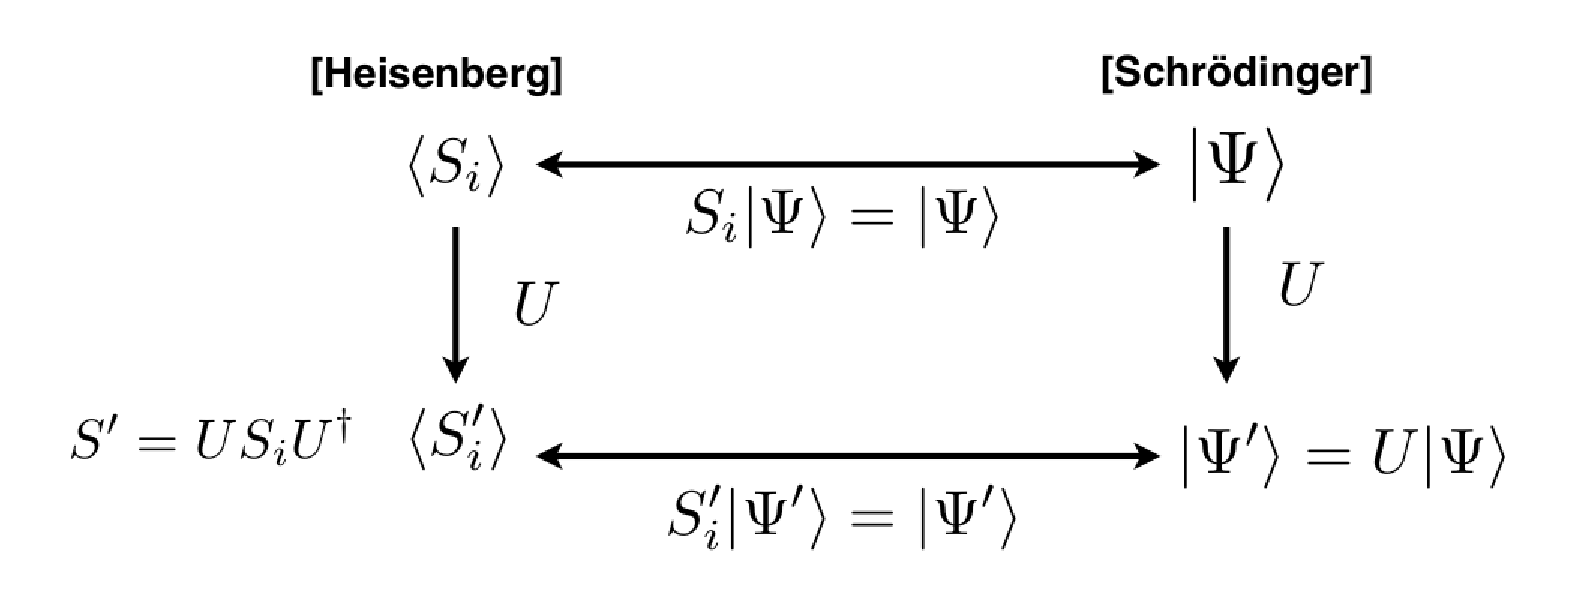
\includegraphics[width=120mm]{fig19.eps}
%
% If not, use
%\picplace{5cm}{2cm} % Give the correct figure height and width in cm
%
\caption{The stabilizer formalism: a Heisenberg picture of quantum computation. A Clifford operation is represented as a transformation of the stabilizer group by the conjugation of $U$.}
\label{fig19}       % Give a unique label
\end{figure}
%%%%%%%%%%%%%%%%%%%%%%%%%%%
%%%%%%%%%%%%%%%%%%%%%%%%%%%
%%%%%%%%%%%%%%%%%%%%%%%%%%%
\section{Clifford operations}
In the stabilizer formalism, 
we can describe a restricted class of unitary operations,
the so-called Clifford operations,\index{Clifford operation}
acting on the stabilizer states quite efficiently.
The Clifford operation is defined as an operation $U$ 
that transforms a Pauli product into another Pauli product under its conjugation, 
$[...] \rightarrow U[...]U^{\dag}$.
Let us consider the action of a Clifford operation\index{Clifford operation} $U$ on the stabilizer state $|\psi \rangle$ defined by a stabilizer group 
$\mathcal{S}=\langle \{S_i\}  \rangle$:
\begin{eqnarray}
U | \psi \rangle = US_i |\psi \rangle  = U S_i U^{\dag}U  | \psi \rangle  = S'_i  U| \psi \rangle,
\end{eqnarray}
where we define $S'_i \equiv U S_i U^{\dag} $.
The above equality indicates that the state $U | \psi \rangle $ is an eigenstate of the operator $S'_i$ with an eigenvalue +1 for all $S'_i$.
Because $U$ is a Clifford (unitary) operation, the group $\{ S'_i \}$ is also an Abelian subgroup of the Pauli group.
Accordingly, the state $U | \psi \rangle $ is a stabilizer state with respect to the stabilizer group $\{ S'_i\}$.
In this way, the action of $U$ on the stabilizer state can be represented as a transformation of the stabilizer groups under the conjugation of $U$ as shown in Fig.~\ref{fig19}.
For example, the stabilizer state stabilized by $\langle X_1I_2, I_1Z_2 \rangle$ is $|+\rangle_1 |0\rangle_2$.
The stabilizer group is transformed by $\Lambda (X)_{1,2}$ into $\langle X_1X_2, Z_1Z_2 \rangle$, whose stabilizer state is $(|00\rangle  + |11\rangle)/\sqrt{2}$.

The stabilizer formalism corresponds to the Heisenberg picture of quantum computation, where a minimum number of operators are employed to describe a restricted type of quantum states and operations~\cite{Gottesman,GottesmanHeisenberg}. 
This representation is powerful because it requires us to keep a time evolution of at most $n$ operators, while a straightforward state-based approach needs exponentially many states.
For example, let us consider the following quantum circuit:
\begin{center}
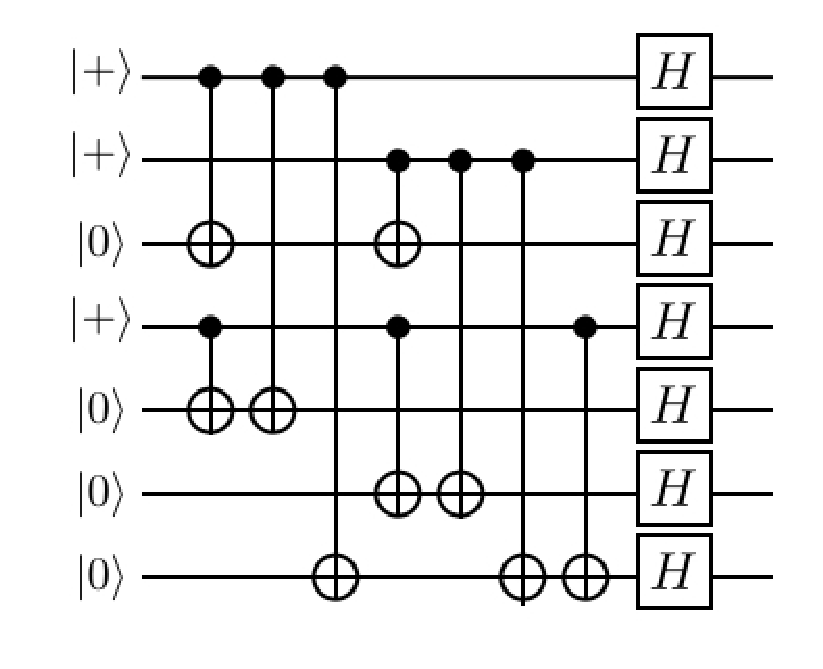
\includegraphics[width=70mm]{fig20.eps}
\end{center}
A straightforward calculation yields the output state $|\psi \rangle$,
\begin{eqnarray}
|\psi \rangle &=& (|0000000\rangle + |1010101\rangle + |0110011\rangle+|1100110\rangle
\nonumber \\
&& + |0001111\rangle + |1011010\rangle+|0111100\rangle+|1101001\rangle 
\nonumber \\
&&+ |1111111\rangle + |0101010\rangle + |1001100\rangle+ |0011001\rangle 
\nonumber \\
&&+ |1110000\rangle + |0100101\rangle+|1000011\rangle+|0010110\rangle)/4.
\end{eqnarray}
It is rather cumbersome to write down the above state.
Instead, we can understand the output state as a stabilizer state whose stabilizer generators are 
\begin{eqnarray}
\{ ZIZIZIZ, IZZIIZZ, IIIZZZZ, XXXIIII, XXIXXII, IXIXIXI, XIIXIIX \}.
\label{eq:7-qubit}
\end{eqnarray}
Equivalently, we may also choose the following stabilizer generators because they generate the same stabilizer group:
\begin{eqnarray}
\{ ZIZIZIZ, IZZIIZZ, IIIZZZZ, XXXXXXX, IIIXXXX, XIXIXIX, IXXIXXI \}.
\end{eqnarray}
Actually, these stabilizer generators are enough to understand the properties of the quantum state $|\psi \rangle$.
If an explicit description of the state is required, we can systematically write it down as follows:
\begin{eqnarray}
|\psi \rangle = 4\frac{I+S_4}{2}\frac{I+S_3}{2}\frac{I+S_2}{2}\frac{I+S_1}{2}|0000000\rangle ,
\end{eqnarray}
where $S_1 = XIXIXIX$, $S_2 = IXXIIXX$, $S_3 = IIIXXXX$, and  $S_4 = XXXXXX$.
The above equation means that $|0000000\rangle$ is an eigenstate for all $Z$'s stabilizer operators.
By projecting it into the $+1$ eigenstate of the stabilizer generator $S_i$ by the projection $\frac{I+S_i}{2}$, we obtain the stabilizer state $|\psi \rangle$.

In order for the above calculation to work, 
we have to obtain the stabilizer generators of the output state.
This can easily be done graphically.
We introduce commutation rules between 
the Pauli operators and Clifford operations below.
In the case of the Hadamard operation, $HX=ZH$ and $ZH=HX$, and hence we have
\begin{center}
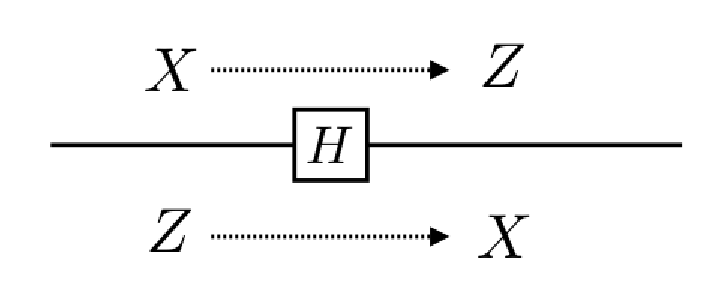
\includegraphics[width=60mm]{fig21.eps}
\end{center}
meaning that the Pauli $X$ operator acting before the Hadamard operation is equivalent to the Pauli $Z$ operator acting after the Hadamard operation and so on.
Similarly, for the phase operation $X$, we have 
\begin{center}
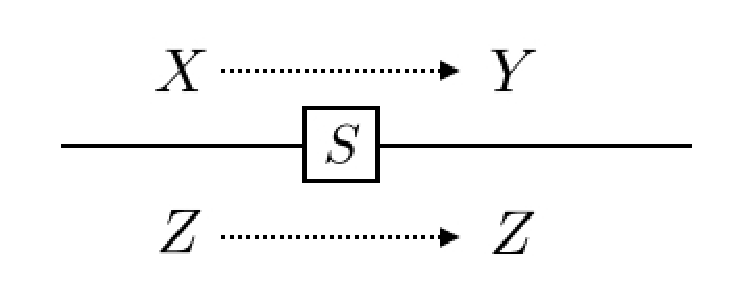
\includegraphics[width=60mm]{fig22.eps}
\end{center}

The CNOT operation transforms the Pauli operators under its conjugation as follows:
\begin{eqnarray}
\Lambda _{c,t} (X) X_c  \Lambda_{c,t}(X) &=& X_c X_t,
\label{eq:CNOT1}
\\
\Lambda _{c,t} (X) X_t  \Lambda_{c,t}(X) &=&  X_t,
\\
\Lambda _{c,t} (X) Z_c  \Lambda_{c,t}(X) &=& Z_c, 
\\
\Lambda _{c,t} (X) Z_t  \Lambda_{c,t}(X) &=& Z_c Z_t.
\label{eq:CNOT4}
\end{eqnarray}
The commutation relation between the CNOT operation and the Pauli operators is understood as follows:
\begin{center}
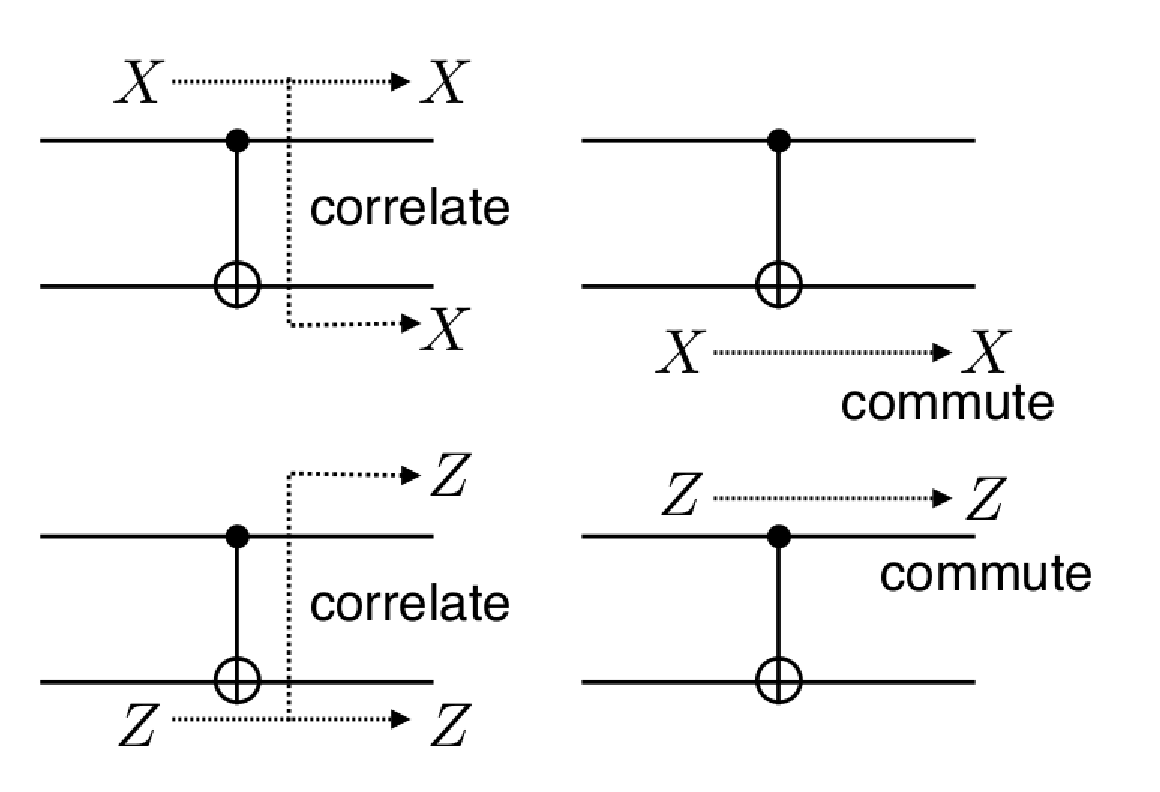
\includegraphics[width=80mm]{fig25.eps}
\end{center}
In the above circuit diagram, the solid circle commutes with the Pauli $Z$ operator, while the Pauli $X$ operator is propagated as the Pauli $X$ operator on the target qubit, making a correlation.
Similarly, the open circle commutes with the Pauli $X$ operator, while the Pauli $Z$ operator is propagated as the Pauli $Z$ operator on the control qubit, making a correlation.
By recalling that the CNOT operation is transformed into the CZ operation by the Hadamard operations on the target qubit, the commutation relation between the CZ operation and the Pauli operators are obtained straightforwardly.
This is described graphically as follows:
\begin{center}
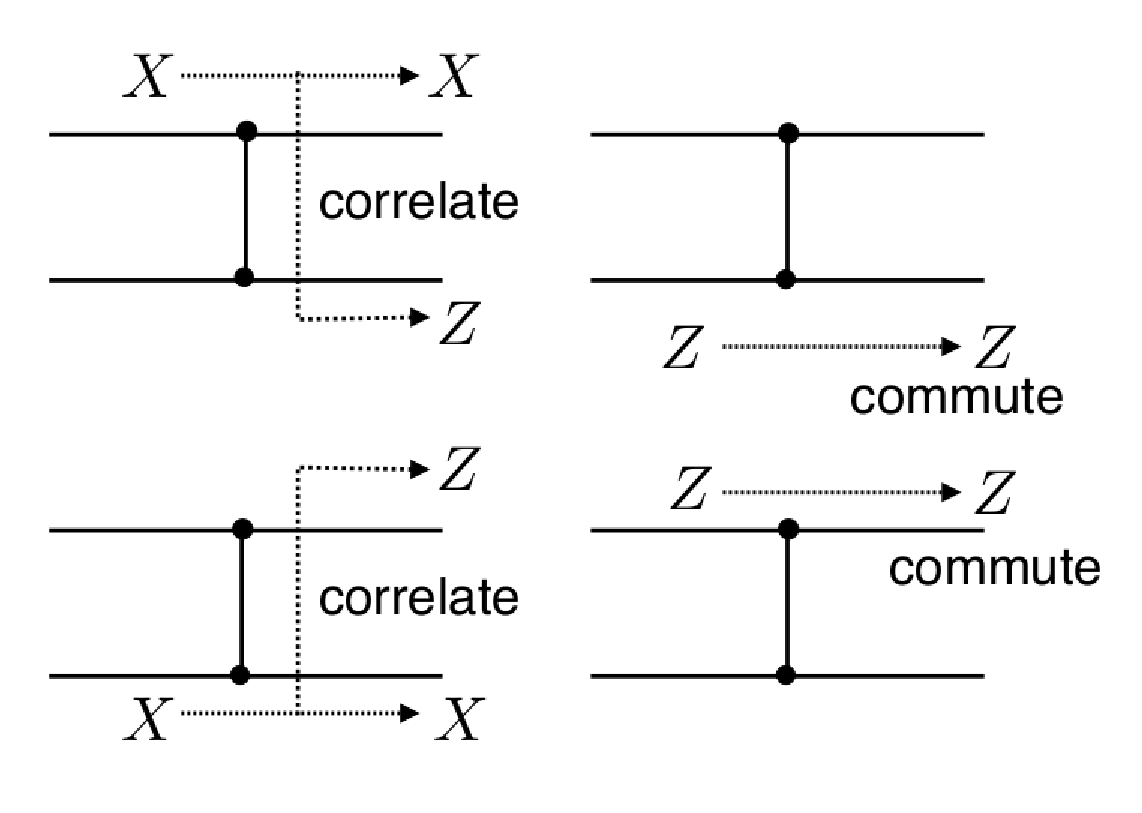
\includegraphics[width=80mm]{fig26.eps}
\end{center}
In this case, note that the Pauli $X$ operation is propagated as the Pauli $Z$ operation.

This graphical understanding allows us to calculate the stabilizer generators of the output of the Clifford circuits.
For example, in the following circuit diagram, the first qubit is stabilized by $X$ before the Clifford operation.
The Pauli $X$ operator is propagated toward the right, and we obtain the stabilizer operator $ZIZIZIZ$ for the output:
\begin{center}
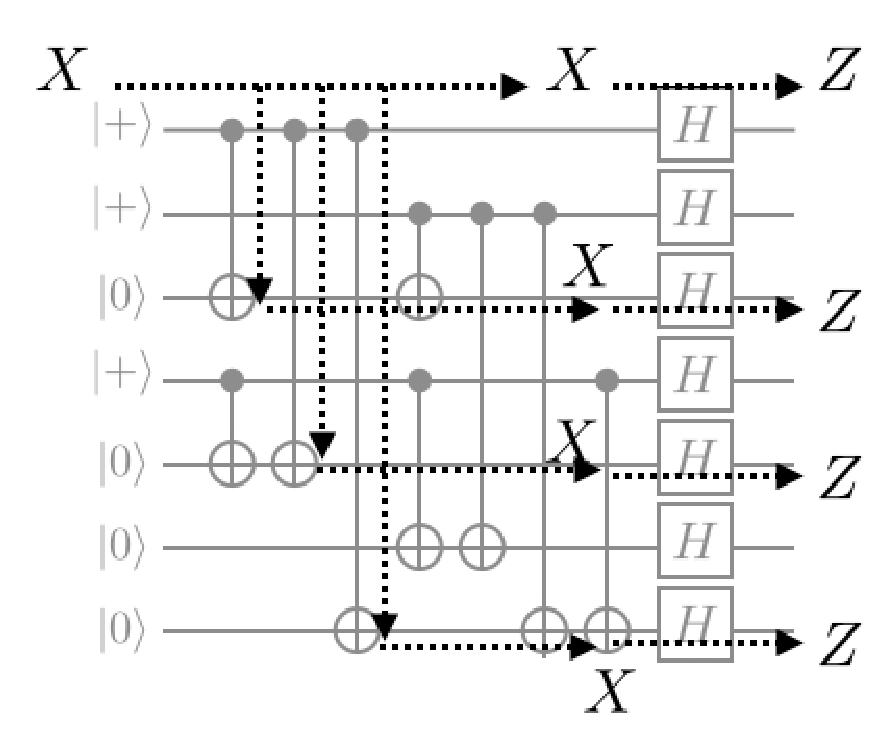
\includegraphics[width=80mm]{fig27.eps}
\end{center}
The reader should use this graphical technique to calculate the other stabilizer generators and verify Eq.\ (\ref{eq:7-qubit}).

%%%%%%%%%%%%%%%%%%%%%%%%%%%
%%%%%%%%%%%%%%%%%%%%%%%%%%%
%%%%%%%%%%%%%%%%%%%%%%%%%%%
\section{Pauli basis measurements}
\label{sec:PauliMeas}
Next, we will see how the Pauli-basis measurements\index{Pauli-basis measurement} on the stabilizer states are described in the stabilizer formalism.
Suppose the $A$-basis ($A=X,Y,Z$) measurement is performed on a stabilizer state $|\psi\rangle$, whose stabilizer group is given by $\langle S_i \rangle$.
(We assume that the number of stabilizer generators is equal to the number of qubits, and hence that the stabilizer state is uniquely defined.)
Depending on the stabilizer group $\langle \{  S_i \} \rangle$ and $A$, there are two possibilities:
\begin{itemize}
	\item[(i)] The Pauli operator $A$ commutes with all stabilizer generators. 
	In that case, either $A$ or $-A$ is an element of the stabilizer group. 
	If $A$ ($-A$) is an element, the eigenvalue $+1$ ($-1$) is obtained with probability 1. 
	The post-measurement state is the same as the stabilizer state before measurement.

	\item[(ii)] At least one stabilizer operator does not commute with $A$. 
	In this case, we can choose another set of generators $\{ S'_i \}$ such that $S'_1$ anti-commutes with $A$ but all other generators commute with $A$. 
	The measurement outcomes $+1$ and $-1$ are obtained with an equal probability of 1/2. The post-measurement state is given by $\langle (-1)^m A, S'_2, ... , S'_k \rangle$ depending on the measurement outcomes $m=0,1$ 
	corresponding to the eigenvalues $(-1)^{m}$.
\end{itemize}

For example, suppose we perform the $Y$-basis measurement on the first qubit of the Bell state stabilized by $\mathcal{S}_{\rm Bell}=\langle XX, ZZ\rangle$.
We can redefine the stabilizer generators by $\{XX, -YY\}$.
Then the stabilizer group after the measurement is given by $\langle YI,-YY \rangle = \langle YI, -IY \rangle$.
Thus, we obtain $|-i\rangle$ as the post-measurement state on the second qubit.

\section{Gottesman-Knill theorem}
\label{sec:GKtheorem}
Because the stabilizer states and Clifford operations are described efficiently in the stabilizer formalism, it implies that such a restricted type of quantum computation can be simulated efficiently on a classical computer.
This is stated by the Gottesman-Knill theorem\index{Gottesman-Knill theorem}~\cite{Gottesman,GottesmanHeisenberg,NielsenChuang}.

\begin{theorem}
Any Clifford operations, applied to the input state $|0\rangle^{\otimes n}$ followed by the $Z$ measurements, can be simulated efficiently in the strong sense.
\label{GKtheorem}
\end{theorem}
Here, an efficient {\it strong} classical simulation of a quantum circuit $C$ is a classical polynomial-time computation that calculates the probability $P_{C}(x)$ 
for a given output $x$ of the circuit $C$,
including an arbitrary marginal distribution $\sum _{x'} P_{C}(x)$. 
(See, for example, Ref.~\cite{IQP} for the definition of a strong simulation.)
Note that this theorem holds true even when the initial state is generalized to an arbitrary stabilizer state, and also any Pauli products are measured, because they are done in the above setup by modifying the Clifford operations appropriately.



%\begin{proof}
{\it Proof:}
The stabilizer group of the input state is $\langle \{ Z_i \} \rangle$
($i=0,1,...,n-1$).
By applying the Clifford operations as mentioned, we obtain the stabilizer generators $\langle \{ S_i \} \rangle$ of the quantum output before the measurements.
Suppose the measurement outcome, the classical output, is given by $\{ m_i=0,1\}$.
Then the probability of obtaining the measurement outcome $\{m_i\}$ can be calculated as follows:
\begin{enumerate}[i)]
	\item Set the stabilizer generators $\mathcal{S}^{(0)} = \langle \{S_i\} \rangle$ and the initial probability $p^{(0)}=1$.

	\item For $k=0,1,...,n-1$, repeat the following procedures.
	\begin{enumerate}[1)]
		\item If $(-1)^{m_k} Z_k \in \mathcal{S}^{(k)}$, update the probability $p^{(k+1)}=p^{(k)}$, because the measurement outcome $m_k$ is obtained with probability $1$. 
		The stabilizer group after the measurement is also updated to $\mathcal{S}^{(k+1)}=\mathcal{S}^{(k)}$.

		\item Else, if $(-1)^{m_k\oplus 1} Z_k \in \mathcal{S}^{(k)}$, update the probability $p^{(k+1)}=0$, because such a measurement outcome does not appear. 
		(You may stop the calculation at this stage, and return the probability 0.)

		\item Else, $\mathcal{S}^{(k)}$ is updated into $\mathcal{S}^{(k+1)}$ by removing an anticommuting generator and adding $(-1)^{m_k} Z_k$ as a new generator. 
		Because the measurement outcome is obtained randomly with probability 1/2, the probability is taken as $p^{(k+1)}=p^{(k)}/2$.
	\end{enumerate}

	\item Return $p^{(n)}$ as the probability of obtaining the measurement outcome $\{ m_i \}$.
\end{enumerate}
Note that, in step (ii), we can efficiently decide which of the three is the case for any $k$ by checking the commutability of $Z_k$ with the stabilizer generators of $\mathcal{S}^{(k)}$.
%\end{proof}
\hfill $\blacksquare$

The statement of Theorem~\ref{GKtheorem} can be extended by weakening the notion of the classical simulation.
\begin{theorem}
Any Clifford operations, applied to any product states of convex mixtures of the Pauli basis states, followed by $Z$ measurements can be efficiently simulated in the weak sense.
\label{GKtheorem_mix}
\end{theorem}
Here, an efficient {\it weak} classical simulation of a quantum circuit $C$ is a classical polynomial-time randomized computation that samples the output $x$ according to the probability distribution $P_{C}(x)$ of the output of the circuit $C$. 
(See, for example, Ref.~\cite{IQP} for the definition of weak simulation.)
Apparently, a strong simulation includes a weak simulation, because we sample the output by using the marginal distributions~\cite{TerhalDiVincenzo}.

{\it Proof:}
Suppose that the $i$th input qubit is given by
\begin{eqnarray}
\rho _{i} &=& p^{(i)}_{x,+} |+\rangle \langle +| +p^{(i)}_{x,-} |-\rangle \langle -| +p^{(i)}_{y,+} |+i\rangle \langle +i| +p^{(i)}_{y,-} |-i\rangle \langle -i|
\nonumber \\
&&+p^{(i)}_{z,+} |0\rangle\langle0|+ p^{(i)}_{z,-} |1\rangle \langle 1|,
\end{eqnarray}
where $\sum _{\alpha =x,y,z} \sum _{\nu = +,-} p_{\alpha , \nu}^{(i)}=1$.
By using the probability distribution $\{p_{\alpha , \nu}^{(i)} \}$, the input state of each qubit is randomly sampled.
Conditioned by the sampling result, the input state is a product of the Pauli basis states, and hence the output probability distribution can be calculated as shown in Theorem~\ref{GKtheorem}.
Combined with the random sampling of the input state, this provides an efficient weak simulation of the Clifford circuit with noisy input states (convex mixture of the Pauli basis states).
\hfill $\blacksquare$
\\
The input state can be generalized into a classical mixture of stabilizer states, when its polynomial size description of the probability distribution is provided. 
Similarly, the Clifford operations can be extended to stochastic Clifford operations such as the stochastic Pauli error.

The convex mixture of the Pauli basis state lies inside the octahedron of the Bloch sphere as shown in Fig.~\ref{fig36}.
It is natural to ask whether or not the Clifford circuit allows universal quantum computation if the input state lies outside the octahedron.
If the input state is a pure non-stabilizer state such as $e^{ - i (\pi/8) Z}|+\rangle$, we can implement a non-Clifford gate $e^{ - i (\pi /8) Z}$ by using gate teleportation, explained in Sec.~\ref{Sec:MBQC}.
Even some mixed states can be converted into a pure non-stabilizer state, the so-called magic state, by using only Clifford operations.
Such a protocol is called magic state distillation~\cite{Magic} and will be explained in Sec.~\ref{sec:magic}.
\begin{figure}[t]
\centering
%\sidecaption
% Use the relevant command for your figure-insertion program
% to insert the figure file.
% For example, with the option graphics use
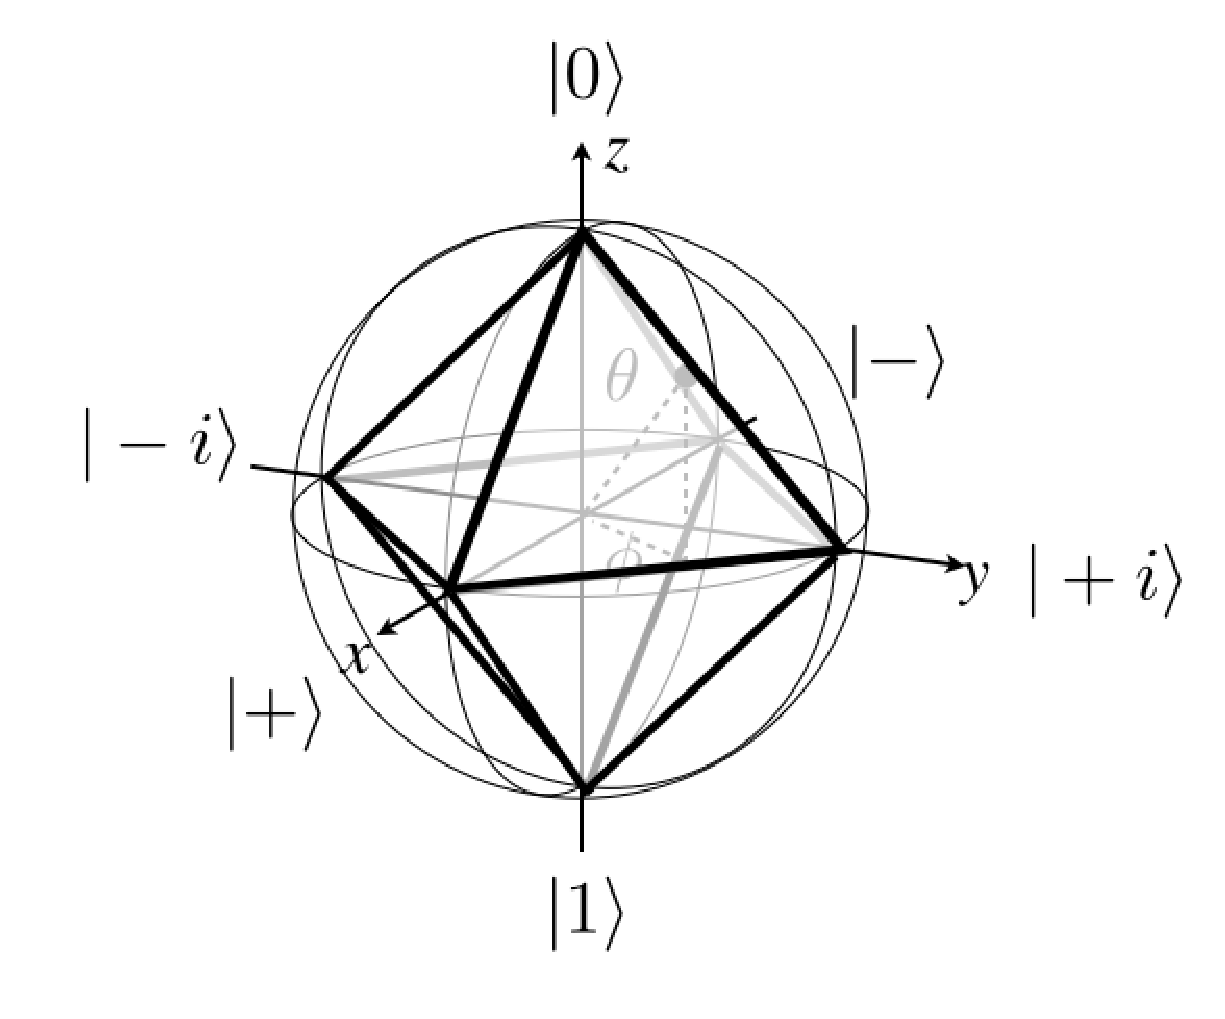
\includegraphics[width=100mm]{fig36.eps}
%
% If not, use
%\picplace{5cm}{2cm} % Give the correct figure height and width in cm
%
\caption{A convex mixture of the Pauli basis states lies inside the octahedron of the Bloch sphere.}
\label{fig36}       % Give a unique label
\end{figure}




%%%%%%%%%%%%%%%%%%
\section{Graph states}
In this section, we introduce an important class of stabilizer states, the so-called {\it graph states}\index{graph state}~\cite{Graphstate}, whose stabilizer generators are defined on graphs.
The graph states are employed as resource states for MBQC as explained in the next section.
\begin{figure}[t]
\centering
%\sidecaption
% Use the relevant command for your figure-insertion program
% to insert the figure file.
% For example, with the option graphics use
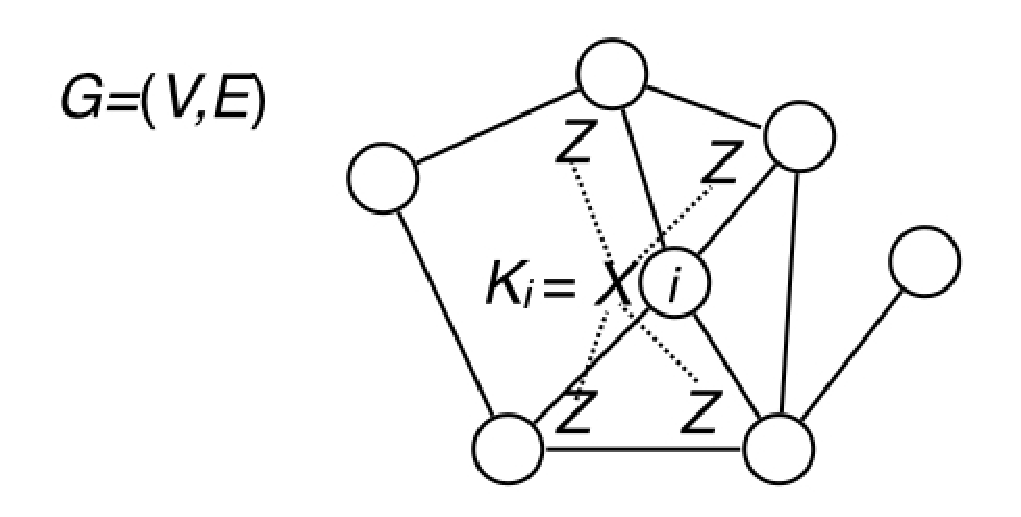
\includegraphics[width=100mm]{fig28.eps}
%
% If not, use
%\picplace{5cm}{2cm} % Give the correct figure height and width in cm
%
\caption{The graph state $|G\rangle$ associated with a graph $G=(V,E)$.
A stabilizer generator $K_i$ is also shown.}
\label{fig28}       % Give a unique label
\end{figure}

A graph state is defined by a graph $G=(V,E)$.
Here, $V$ and $E$ are the sets of the vertices and edges, respectively.
A qubit is located on each vertex of the graph.
The stabilizer generator of the graph state $|{G}\rangle$ is defined as
\begin{eqnarray}
K_i =  X_i \prod _{ j \in V_i } Z_j \;\; \textrm {for all } i \in V ,
\end{eqnarray}
where we define a set of vertices $V_i:= \{ j | (i,j) \in E \}$, which are connected to the vertex $i$ by an edge on the graph $G$ (see Fig.~\ref{fig36}).
The graph state $|G\rangle$ is generated from a product state $|+\rangle^{\otimes |V|}$ by applying the CZ gate on each of the graphs:
\begin{eqnarray}
|G\rangle = \prod _{(i,j) \in E} \Lambda (Z)_{i,j} | +\rangle^{\otimes |V|},
\end{eqnarray}
where $|V|$ indicates the number of vertices of the graph $G=(V,E)$.
This can be understood that the stabilizer generator $X_i$ for the state $|+\rangle$ is transformed into $K_i$ by the CZ operations $U\equiv \prod _{(i,j) \in E} \Lambda (Z)_{i,j}$.
Especially, when the graphs are regular lattices such as one-dimensional (1D), square, hexagonal, and cubic lattices, the corresponding graph states tend to be referred to as cluster states\index{cluster states}~\cite{Cluster}.
Any stabilizer state is equivalent to a certain graph state up to local Clifford operations~\cite{LCeq,Graphstate}. 
For example, the cat state is equivalent to the following graph state by applying the Hadamard operation on the $k$th qubit:
\begin{center}
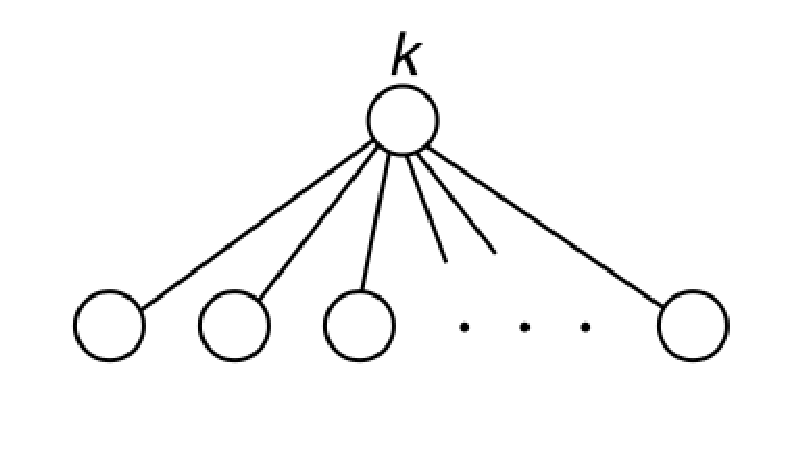
\includegraphics[width=60mm]{fig29.eps}
\end{center}
Unfortunately, the graph associated with a stabilizer state is not uniquely defined, because there are local Clifford operations that change the underlying graph.
This property is called the local complementarity of the graph states~\cite{LCeq,Graphstate}.

Next, we will see how the Pauli basis measurements transform the graph states.
For simplicity, we assume that the state is projected into an eigenstate with eigenvalue $+1$.
Let us consider a 1D graph state as follows:
\begin{center}
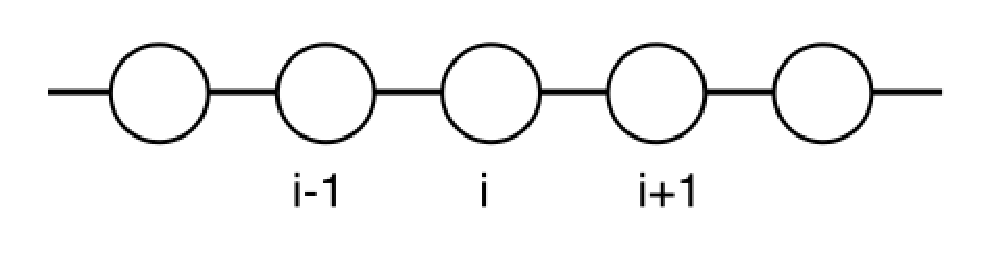
\includegraphics[width=70mm]{fig30.eps}
\end{center}
whose stabilizer generator is given by
\begin{eqnarray}
K_i=Z_{i-1}X_i Z_{{i+1}}.
\end{eqnarray}
We first consider the $Z$ basis measurement (projective measurement of the observable $Z$) on the $i$th qubit. 
Following the procedure seen in Sec.~\ref{sec:PauliMeas}, $K_i$ is removed from the stabilizer generator.
By adding $Z_i$ instead, we obtain the stabilizer group for the post-measurement state
\begin{eqnarray}
\langle ..., K_{i -1}, Z_{i}, K_{i+1} ,...\rangle.
\end{eqnarray}
After the projection, the $i$th qubit is $|0\rangle$ and hence decoupled from the other qubits.
By rewriting the stabilizer generators, we obtain three decoupled stabilizer groups
\begin{eqnarray}
\langle ..., Z_{i-2}X_{i-1}  \rangle  , \langle Z_i \rangle, \langle   X_{i+1} Z_{i+2} ,...\rangle.
\end{eqnarray}
This means that the graph is divided into two parts as follows:
\begin{center}
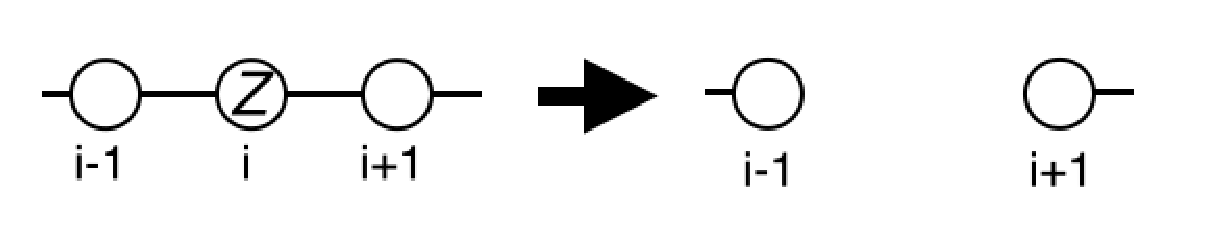
\includegraphics[width=90mm]{fig31.eps}
\end{center}
For any graph, this property of the $Z$-basis measurement holds; the post-measurement state is defined by a modified graph, where the vertex corresponding to the measured qubit and the edges incident to it are removed from the original graph.

Next, we consider the $X$-basis measurement.
The observable $X_i$ does not commute with $K_{i-1}$ and $K_{i+1}$, but does commute with $K_{i-1}K_{i+1}=Z_{i-2} X_{i-1}X_{i+1} Z_{i+2}$.
Following the procedure in Sec.~\ref{sec:PauliMeas}, the stabilizer group for the post-measurement state is calculated to be
\begin{eqnarray}
\langle ...,Z_{i-2} X_{i-1}X_{i+1} Z_{i+2}, Z_{i-1}Z_{i+1}  ,...\rangle, \langle X_i \rangle.
\end{eqnarray}
By performing the Hadamard operation $H$ on the $(i-1)$th qubit, we obtain a new stabilizer group 
\begin{eqnarray}
\langle ...,Z_{i-2} Z_{i-1}X_{i+1} Z_{i+2}, X_{i-1}Z_{i+1}  ,...\rangle, \langle X_i \rangle,
\end{eqnarray}
which indicates that the graph is transformed into the following graph with the Hadamard operation:
\begin{center}
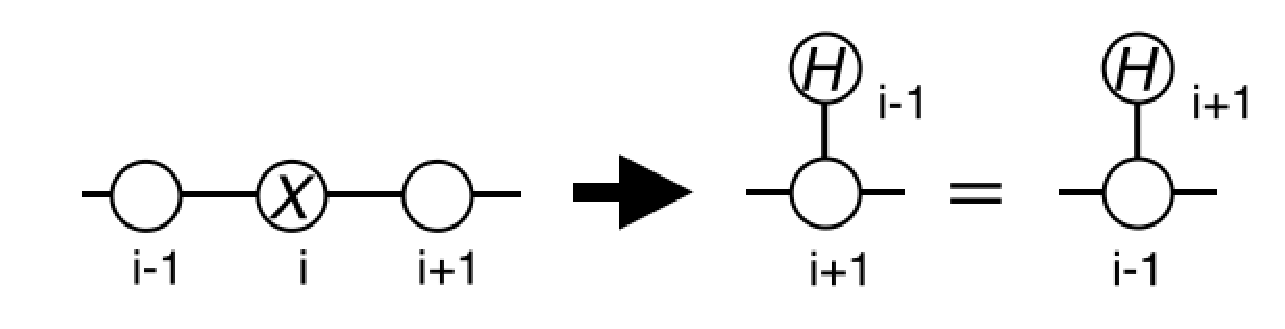
\includegraphics[width=90mm]{fig32.eps}
\end{center}
Instead of the $(i-1)$th qubit, we can obtain a similar result by performing the Hadamard operation on the $(i+1)$th qubit as shown above.

Suppose the $i$th and $(i+1)$th qubits are measured in the $X$-basis on a 1D graph state. 
This is equivalent to measuring the $(i+1)$th qubit of the above post-measurement graph state in the $Z$ basis, because the Hadamard operation is applied on it as a byproduct.
From the previous argument, the $Z$-basis measurement remove the measured qubit from the graph.
Thus, two neighboring $X$-basis measurements remove the measured qubits and connect the left and right hand sides directly:
\begin{center}
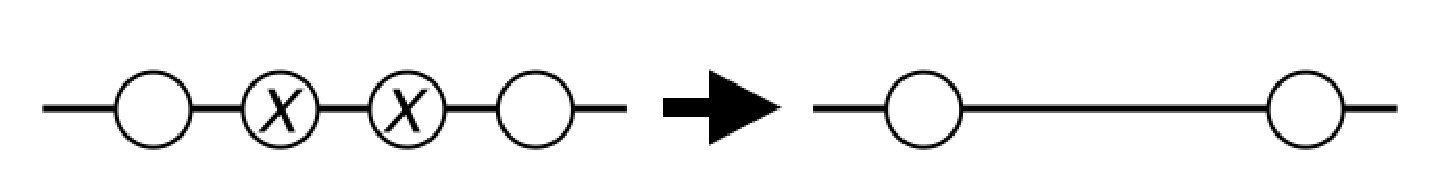
\includegraphics[width=90mm]{fig34.eps}
\end{center}
which we call a contraction.

Finally, we consider the $Y$-basis measurement.
The observable $Y_i$ does not commute with either $K_{i-1}$, $K_i$, or $K_{i+1}$, but does commute with $K_{i-1}K_{i}= Z_{i-2} Y_{i-1} Y_i Z_{i+1} $ and 
$K_{i}K_{i+1}= Z_{i-1} Y_{i} Y_{i+1} Z_{i+2} $.
The stabilizer group for the post-measurement state is calculated to be
\begin{eqnarray}
\langle ...,Z_{i-2} Y_{i-1} Z_{i+1}, Z_{i-1} Y_{i+1} Z_{i+2}  ,...\rangle, \langle Y_i \rangle.
\end{eqnarray}
By performing the phase gates $S$ on the $(i-1)$th and $(i+1)$th qubits, we obtain a new stabilizer group
\begin{eqnarray}
\langle ...,Z_{i-2} X_{i-1} Z_{i+1}, Z_{i-1} X_{i+1} Z_{i+2}  ,...\rangle, \langle Y_i \rangle.
\end{eqnarray}
This indicates that the graph is directly connected up to the phase operation $S$ as a byproduct:
\begin{center}
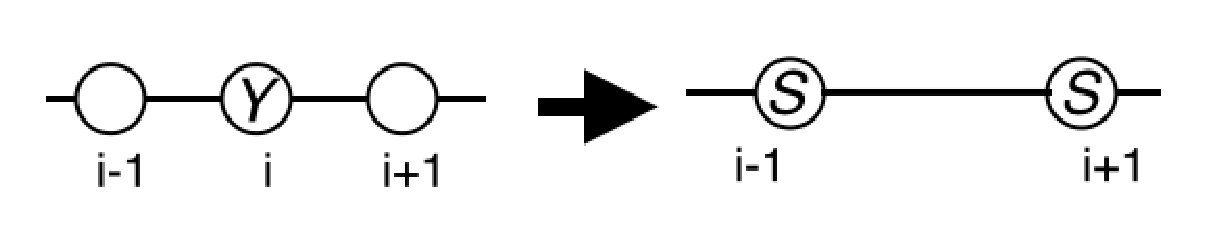
\includegraphics[width=90mm]{fig33.eps}
\end{center}

Suppose three neighboring qubits $(i-1)$, $i$, and $(i+1)$ are measured in the $Y$-basis.
This is equivalent to measuring the $i$th qubit in the $Y$-basis, and then measuring the $(i-1)$th and $(i+1)$th qubits of the post-measurement graph state in the $X$-basis, because there is a phase operation $S$ acting on them as a product.
As seen previously, the $X$-basis measurements on two neighboring qubits result in a contraction of the two qubits on the graph.
Thus, the $Y$-basis measurements on three neighboring qubits contract them from the 1D graph state.
\begin{center}
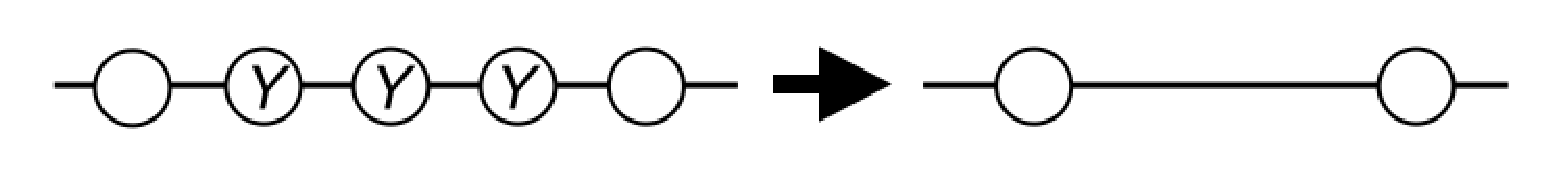
\includegraphics[width=90mm]{fig35.eps}
\end{center}
This property is useful to change even and odd of the length of the 1D graph state.

While we have considered the Pauli-basis measurements only on the 1D graph state, we can generalize these arguments into graph states of general structures.
A graph state is still mapped into another graph state up to some single-qubit Clifford operations as byproducts.



\section{Measurement-based quantum computation}
\label{Sec:MBQC}
Measurement-based quantum computation (MBQC)\index{measurement-based quantum computation} is a model of quantum computation, where quantum gates are implemented by adoptive measurements on a highly entangled resource state~\cite{MBQC,MBQC_PRA,RaussendorfPhD}. 
Specifically, certain graph states, the so-called cluster states, are employed as resource states in MBQC.
Below we will first demonstrate quantum teleportation, a building block of MBQC.
Then, we explain how adoptive measurements on a graph state enable us to emulate universal quantum computation via quantum teleportation. 

%\subsubsection*{Quantum teleportation}
Quantum teleportation is a quantum communication protocol, in which Alice sends a quantum state to Bob by using a shared entangled state and classical communication~\cite{teleportation}.
Suppose Alice and Bob share a maximally entangled state, the Bell state, 
\begin{eqnarray}
\frac{|0\rangle _a |0\rangle _b + |1\rangle _a |1\rangle _b}{\sqrt{2}}.
\end{eqnarray}
For an unknown input state $|\psi \rangle_i$ and the half of the Bell state, Alice performs a Bell measurement, which is a projection onto the Bell basis states
\begin{eqnarray}
|\Psi(m_1,m_2)\rangle _{i,a} = X^{m_1}_i Z_i^{m_2}\frac{|0\rangle _i |0\rangle _a + |1\rangle _i |1\rangle _a}{\sqrt{2}},
\end{eqnarray}
where $m_1,m_2 =0,1$ correspond to the measurement outcomes.
A straightforward calculation provides
\begin{eqnarray}
\langle \Psi(m_1,m_2) |_{i,a} \left( |\psi \rangle _i \frac{|0\rangle _a |0\rangle _b + |1\rangle _a |1\rangle _b}{\sqrt{2}} \right)
=Z^{m_2}_b X^{m_1}_b  |\psi \rangle _{b}/2.
\end{eqnarray} 
Hence, the unknown input state is teleported to Bob with a byproduct operator\index{byproduct operator} $X^{m_1} Z^{m_2}$.
If Bob does not know the measurement outcomes $(m_1,m_2)$, the teleported state is a completely mixed state for Bob.
However, if Alice sends the measurement outcome as a classical message, Bob can undo the byproduct and obtain the unknown quantum state at Bob's side.
The circuit diagram of quantum teleportation is:
\begin{center}
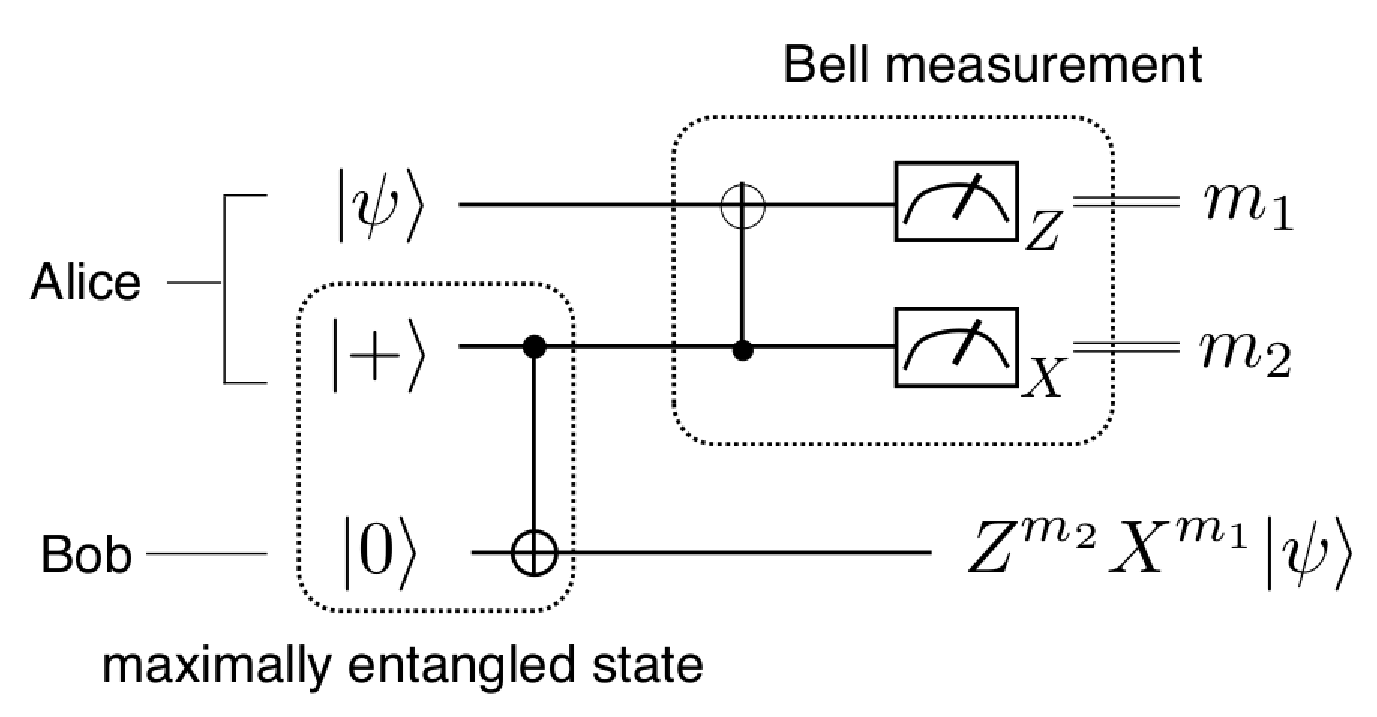
\includegraphics[width=100mm]{fig17.eps}
\end{center}
By using the following circuit equivalence, we can decompose the teleportation circuit into two elementary teleportations, the so-called {\it one-bit teleportations}\index{one-bit teleportation}:
\begin{center}
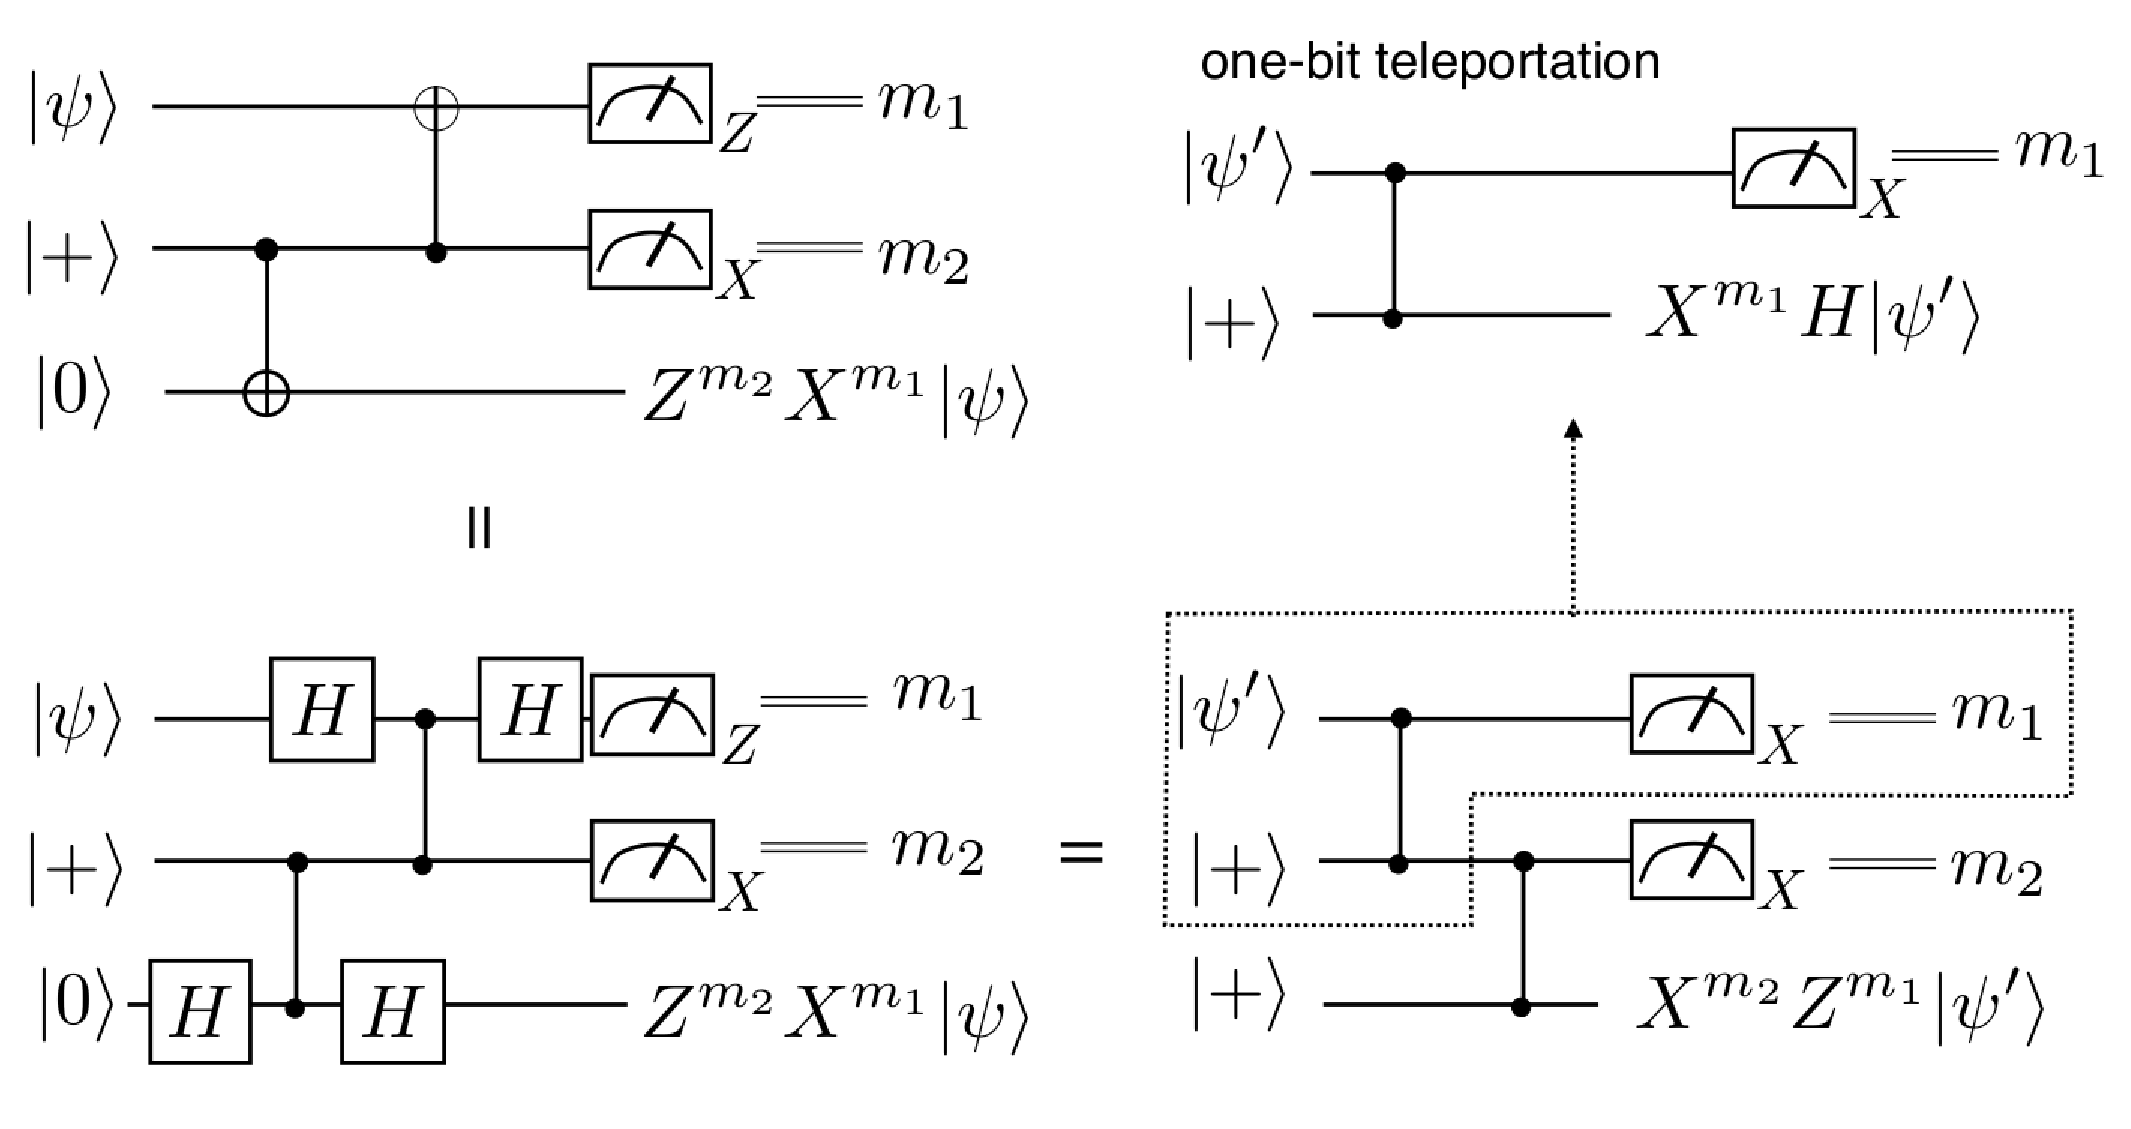
\includegraphics[width=130mm]{fig18.eps}
\end{center}
One-bit teleportation is useful as a building block of the teleportation-based gates employed in MBQC.
A single-qubit $Z$ rotation $e^{i\theta Z}$ can be implemented in a teleportation-based way.
Its action can be understood from the following circuit equivalence:
\begin{center}
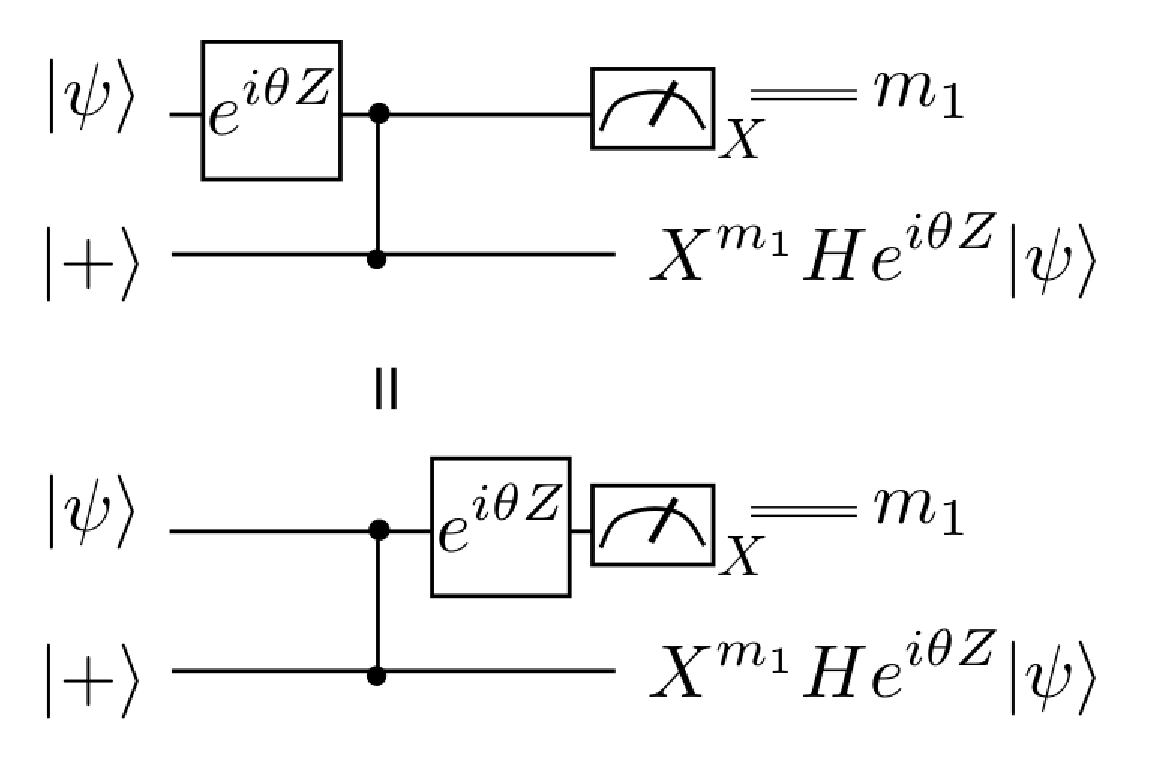
\includegraphics[width=80mm]{fig23.eps}
\end{center}
where we utilized the fact that $e^{i\theta Z}$ and $\Lambda(Z)$ commute.
The controlled-$Z$ operation is also implemented in a teleportation-based way as follows:
\begin{center}
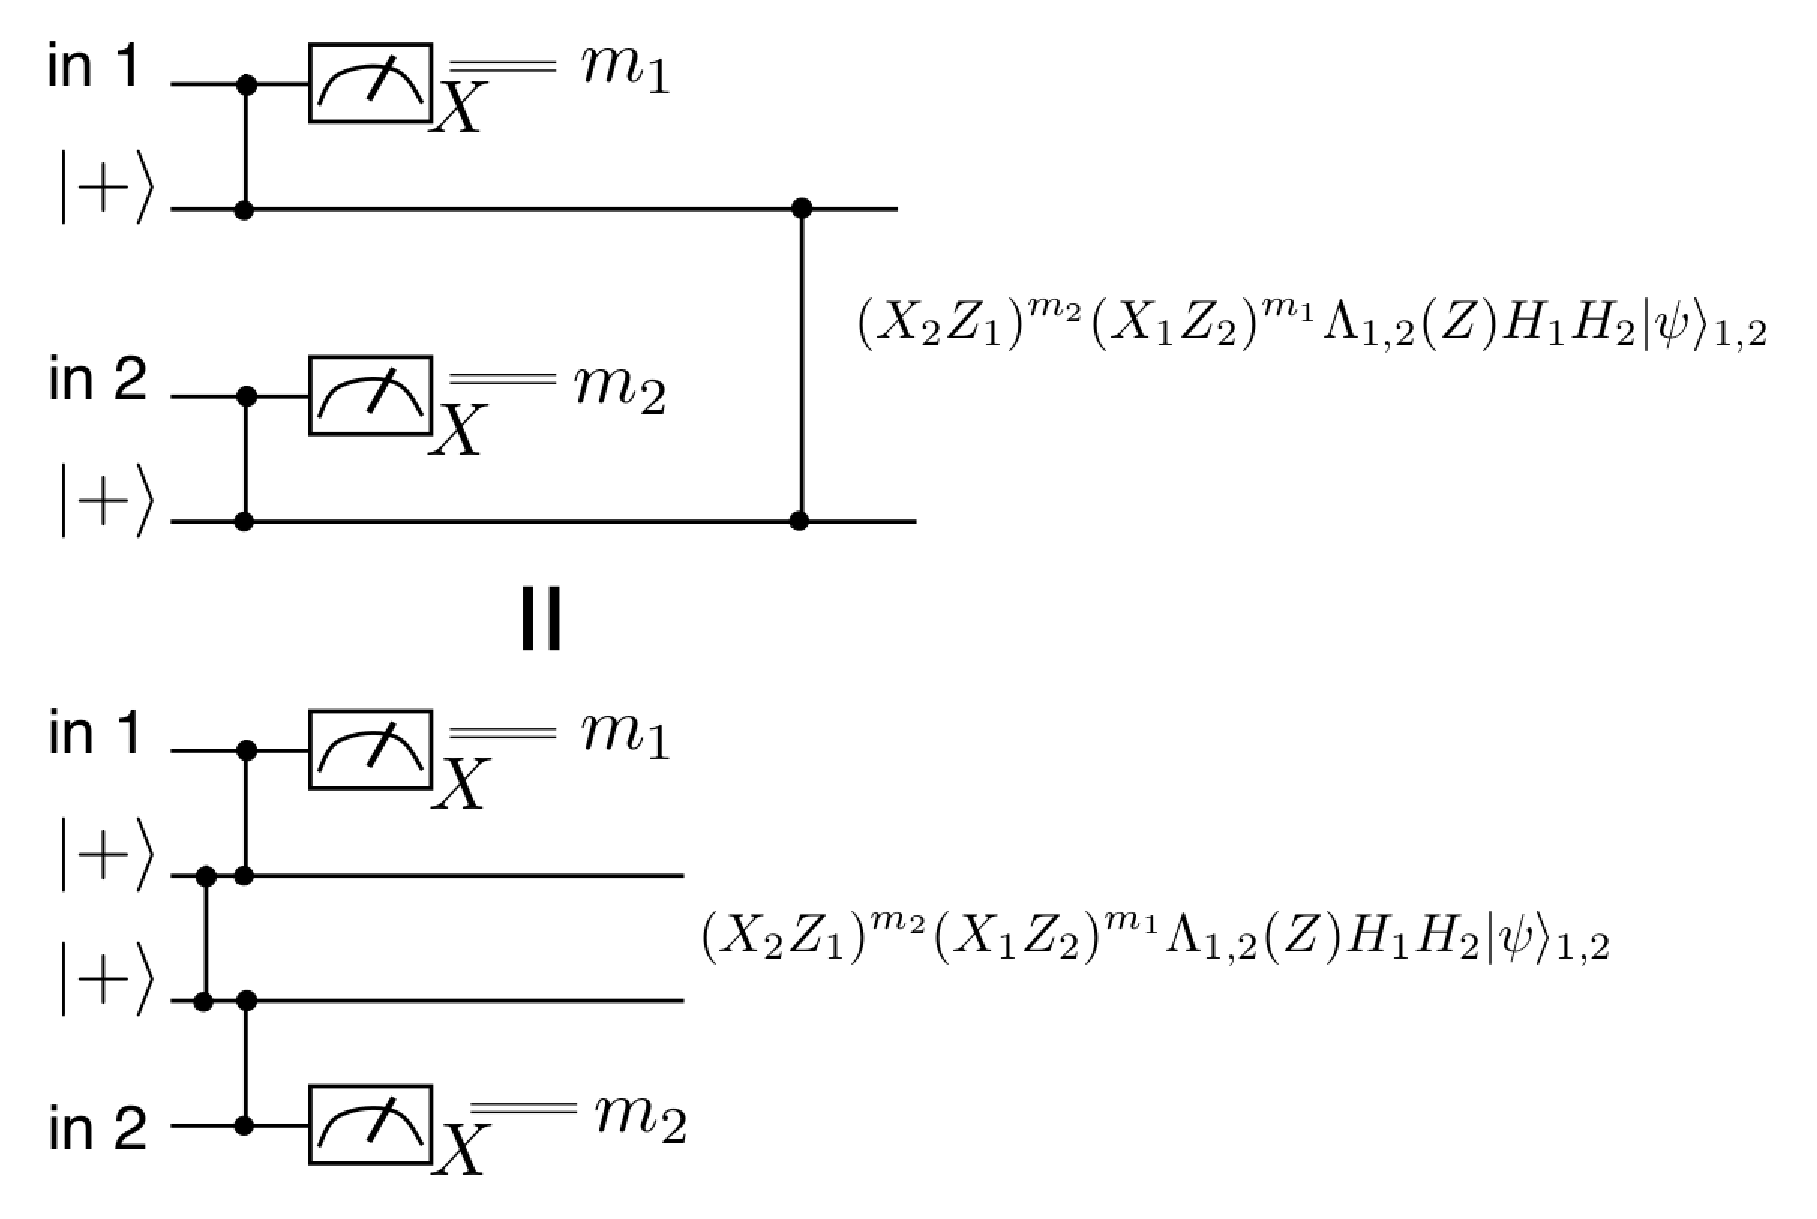
\includegraphics[width=120mm]{fig24.eps}
\end{center}
That is, instead of performing the $\Lambda(Z)$ gate after one-bit teleportations, we can prepare a special resource state, on which the $\Lambda(Z)$ gate is pre-implemented, and the $\Lambda(Z)$ gate is then performed via teleportation.
These quantum operations based on quantum teleportation are called {\it gate teleportation}\index{gate teleportation}~\cite{GottesmanChuang}.

Now we are ready to formulate MBQC.
An arbitrary single-qubit unitary operation $U$ can be decomposed, up to an unimportant global phase, into 
\begin{eqnarray}
U &=& He^{i \phi Z} e^{i \theta X} e^{i \xi Z}
\\
&=&He^{i \phi Z} He^{i \theta Z} He^{i \xi Z}.
\end{eqnarray}
This indicates that we can perform an arbitrary single-qubit unitary operation by a sequence of one-bit teleportations.
The resource state for the sequential one-bit teleportations is a 1D cluster state: 
\begin{center}
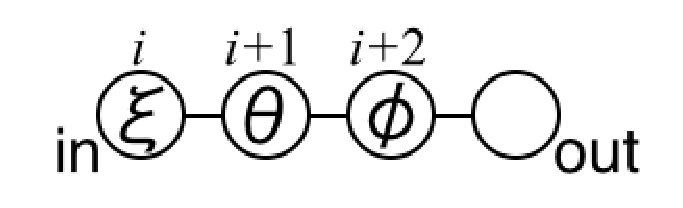
\includegraphics[width=50mm]{fig37.eps}
\end{center}
where the stabilizer generator for the left-most qubit is removed and the input state is encoded.
We have to take care of the byproduct Pauli operators depending on the measurement outcomes.
Fortunately, we can propagate the Pauli byproduct operators\index{byproduct operator} forward as follows:
\begin{eqnarray}
U&=& X^{m_{i+2}}He^{i \phi'  Z} X^{m_{i+1}} He^{i \theta' Z}  X^{m_i} He^{i \xi Z}.
\\
&=& X^{m_{i+2}\oplus m_{i}}Z^{m_{i+1}} He^{i(-1)^{m_{i+1}} \phi'  Z} He^{i (-1)^{m_i}\theta' Z} He^{i \xi Z}.
\end{eqnarray}
\begin{center}
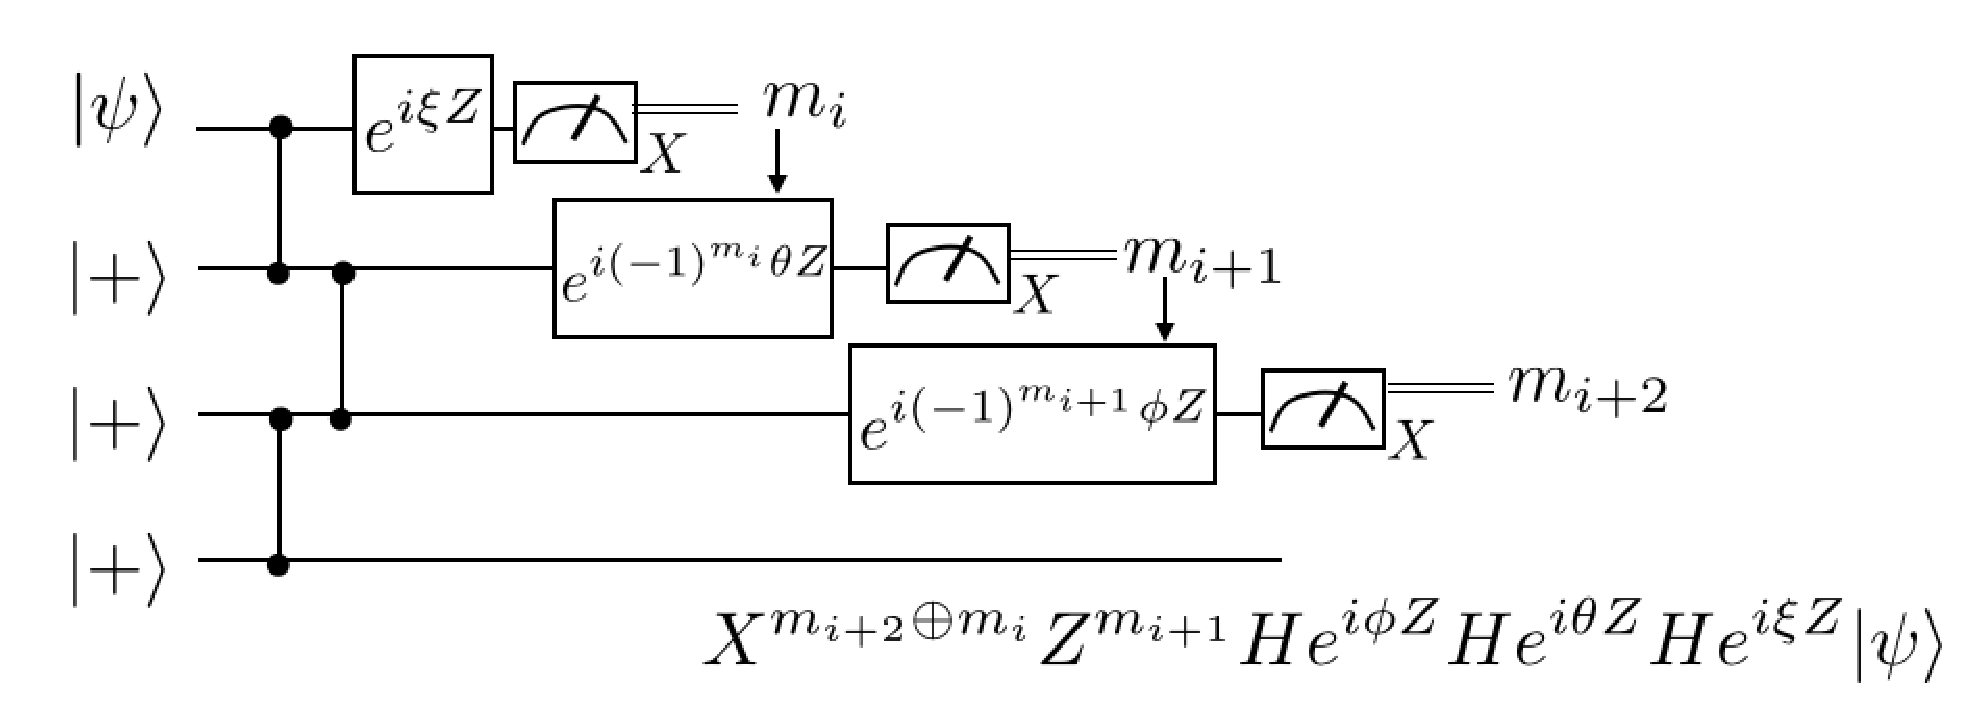
\includegraphics[width=120mm]{fig38.eps}
\end{center}
By choosing $\theta ' = (-1)^{m_i} \theta $ and $\phi' = (-1)^{m_{i+1}} \phi$ adaptively, depending on the previous measurement outcomes, the random nature of the measurements can be managed.
This procedure is called {\it feedforward}\index{feedforward}.
The Pauli byproduct is propagated and updated throughout the computation.
Note that the classical processing required to determine the measurement angle has only XOR (addition modulo two) operations~\cite{MBQC_PRA}. 

Next, we will investigate the measurement-based two-qubit gate operation.
The resource state for the gate teleportation\index{gate teleportation} is the following cluster state:
\begin{center}
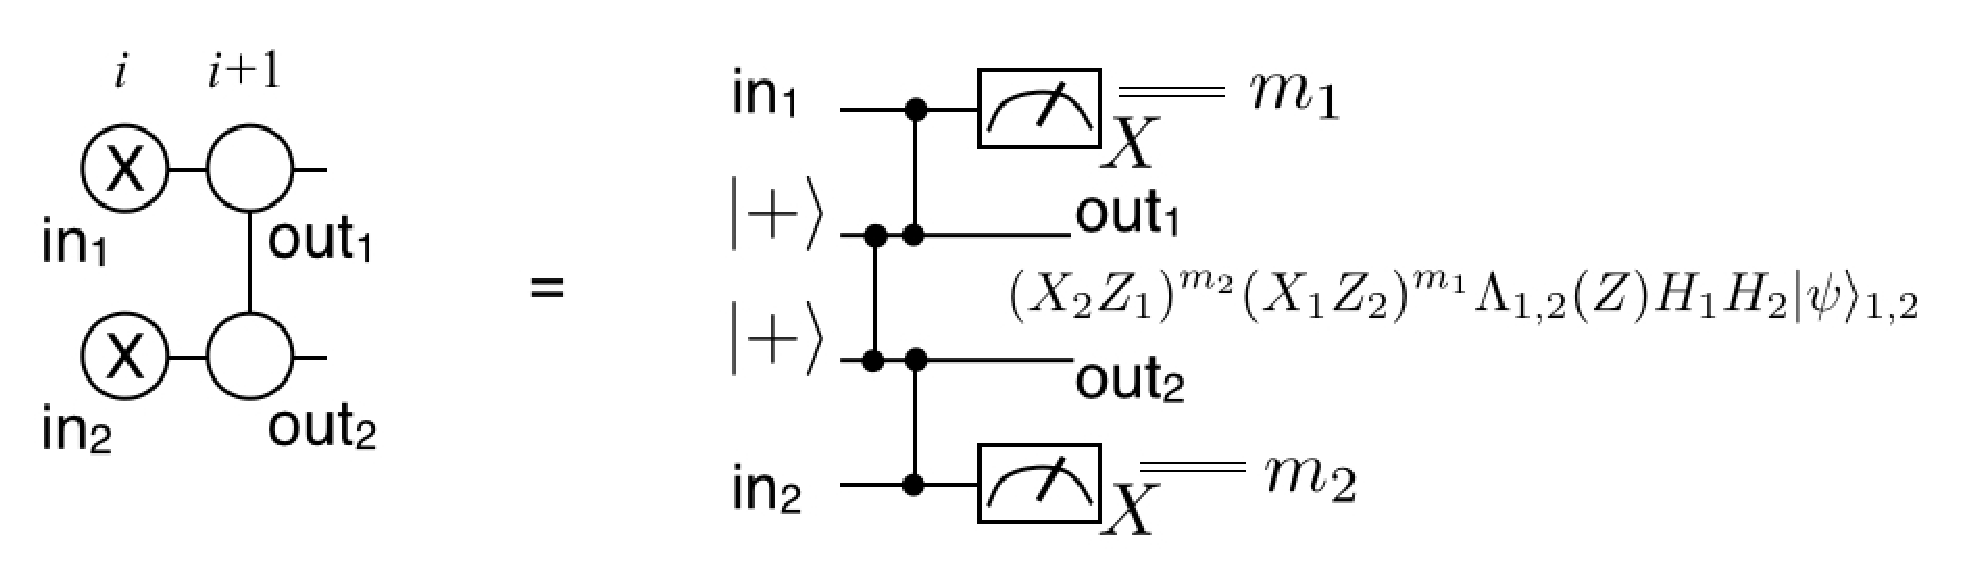
\includegraphics[width=120mm]{fig40.eps}
\end{center}
To adjust the timing of the two-qubit operation, we can insert identity operations depending on the even and odd lengths as follows:
\begin{center}
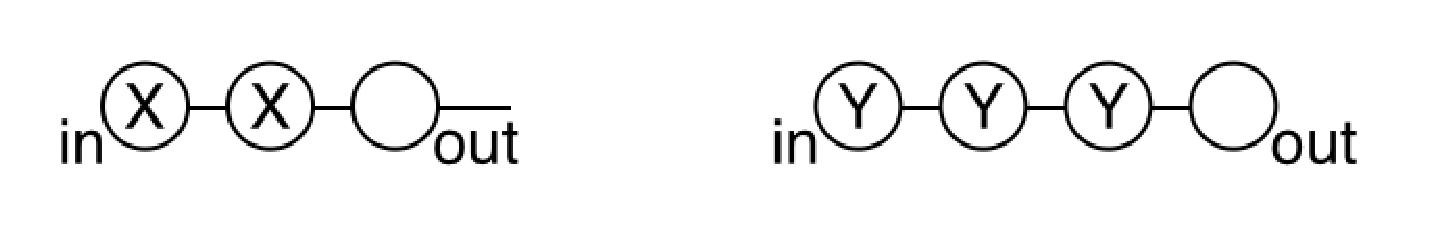
\includegraphics[width=100mm]{fig39.eps}
\end{center}
Without loss of generality, we can assume that all input states of the quantum computation are given by $|+\rangle$, which are automatically encoded by preparing the graph state.
At the end of the computation (on the right-most qubits), measurements are performed to read out the result as follows:
\begin{center}
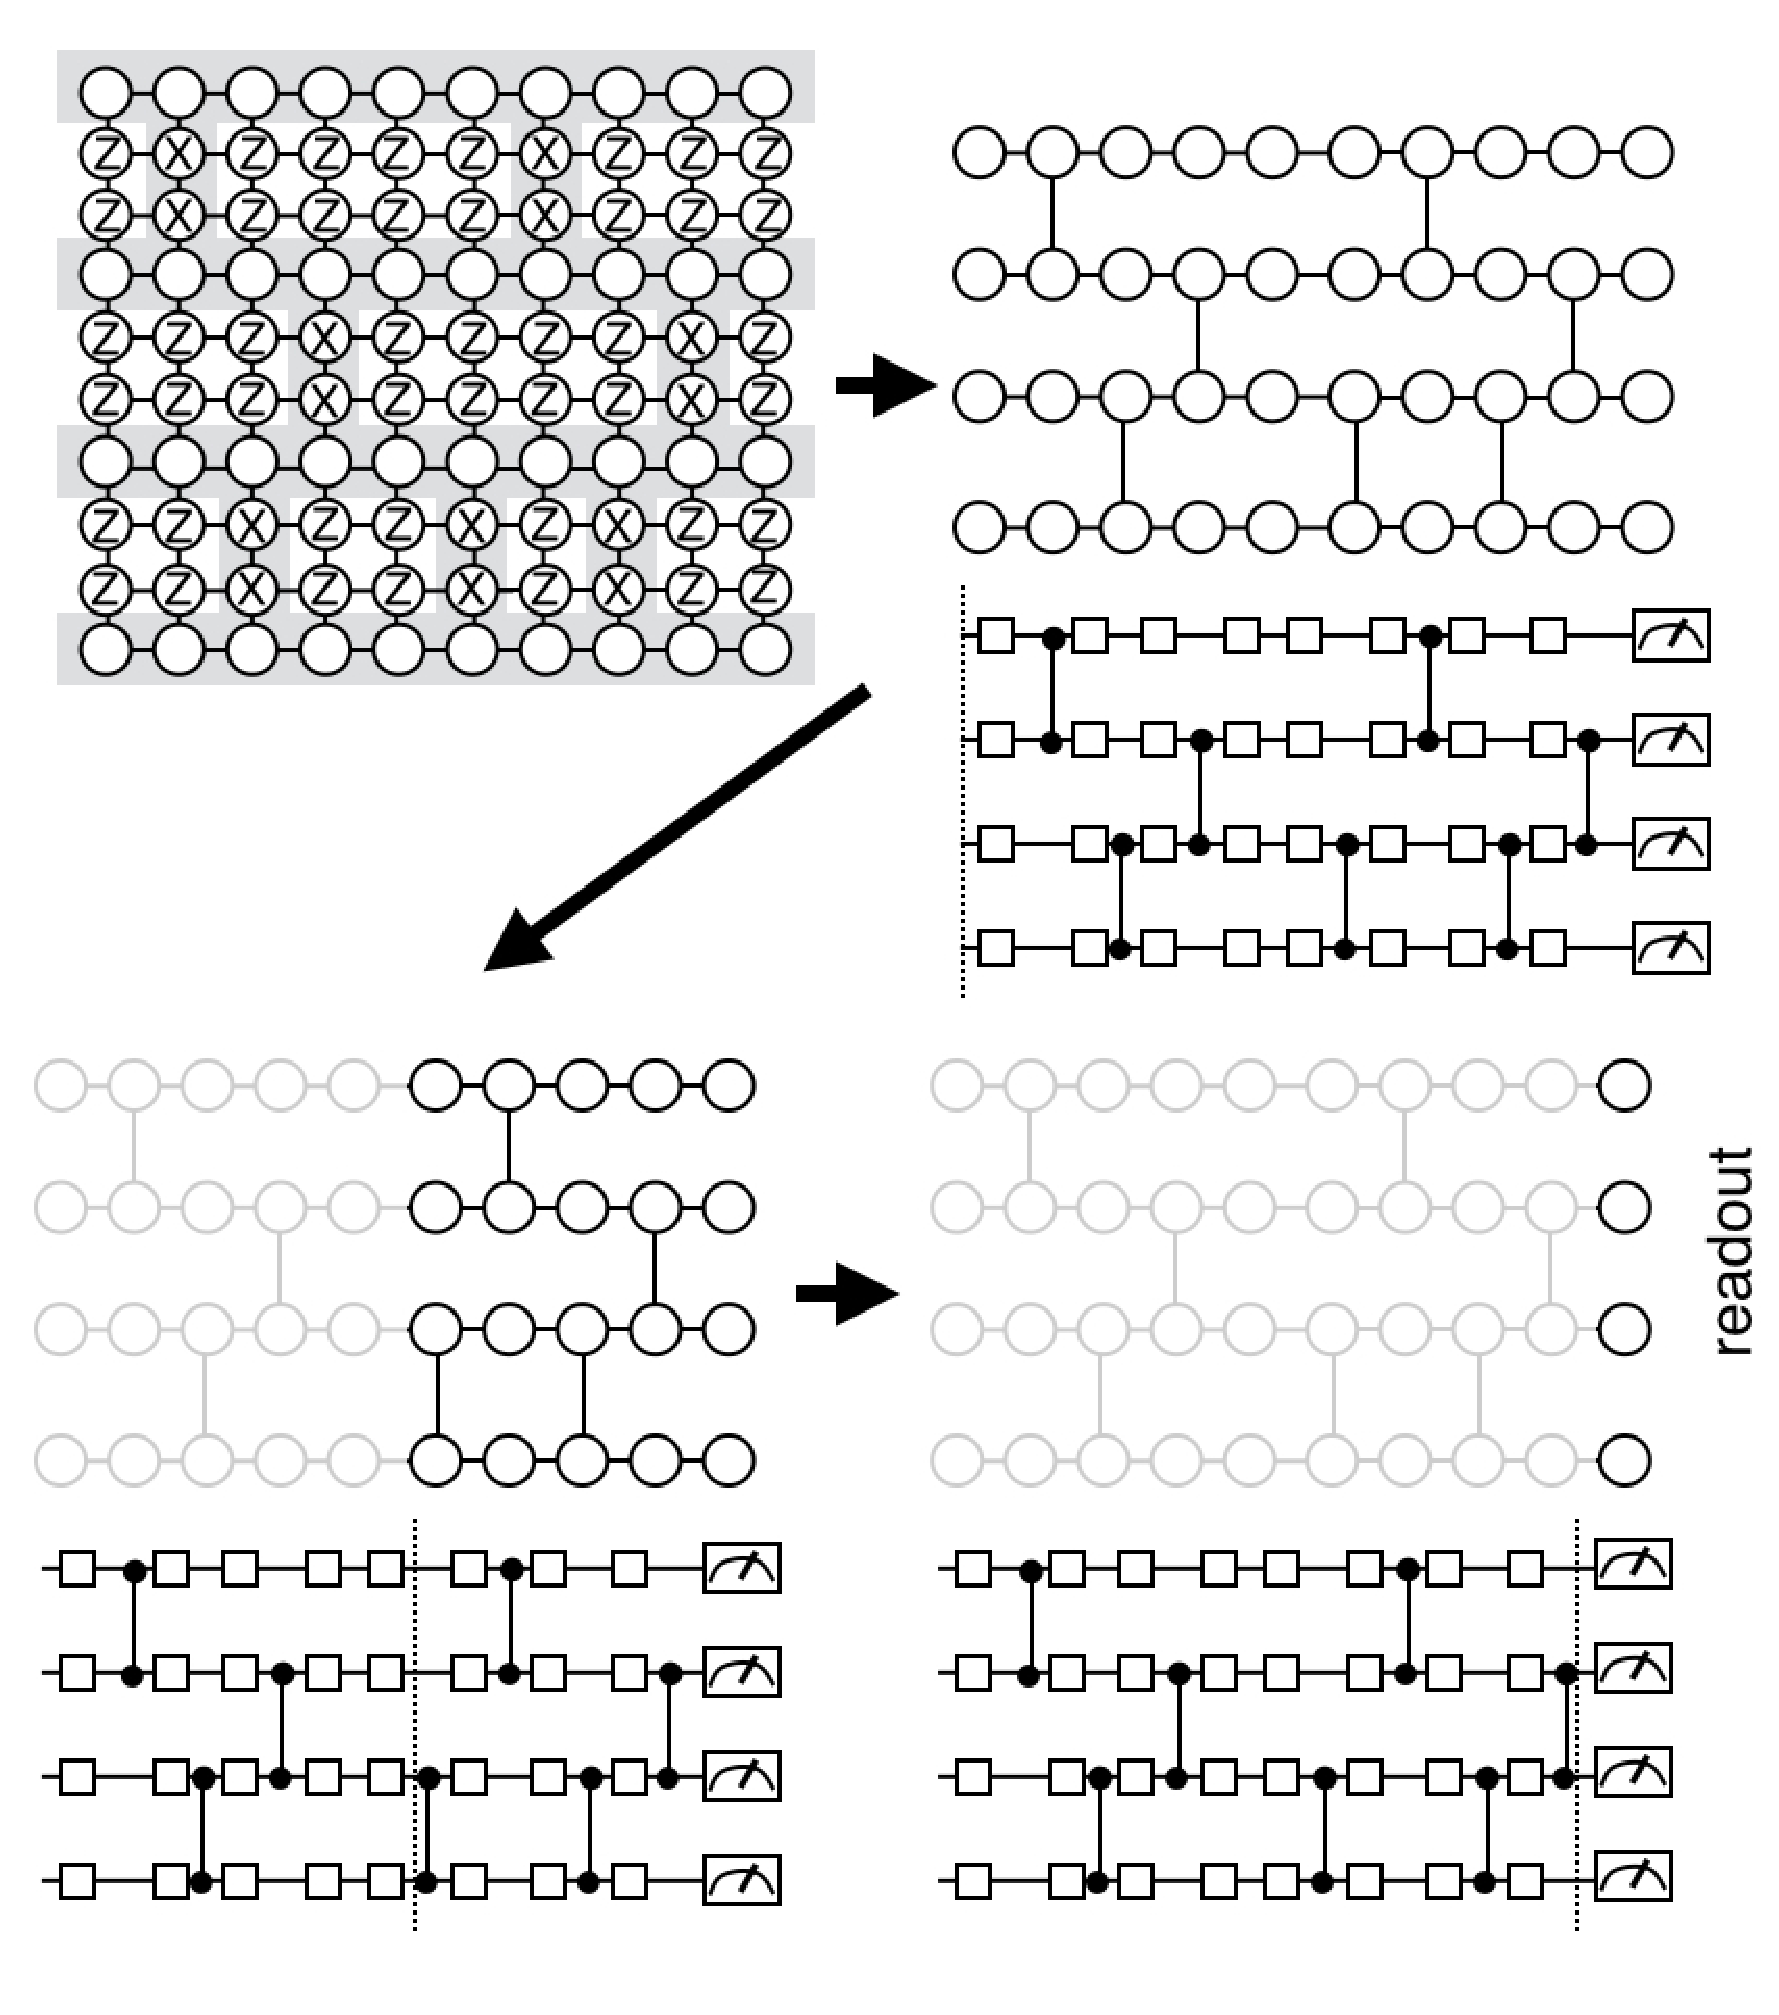
\includegraphics[width=100mm]{fig41.eps}
\end{center}
In this way, universal quantum computation is simulated solely by measurements on a brickwork-like cluster state.
This state can be generated from a cluster state on a square lattice by using the Pauli basis measurements as shown above.
Accordingly, the square lattice cluster states are universal resources for MBQC.

The above circuit-based explanation of MBQC~\cite{NielsenCluster} is very intuitive and straightforward.
However, for a complicated resource state, as will be shown, an operator-based understanding of MBQC~\cite{MBQC_PRA} is quite useful.
Let us reformulate MBQC from an operator viewpoint.
Suppose again an MBQC on a 1D cluster state.
The measurements are executed up to the $(i-1)$th qubits, and hence the operator $K_l$ ($l \leq i$) is removed from the stabilizer generators.
The logical degree of freedom on the remaining resource state can be specified by the $i$th logical operators\index{logical operator}
\begin{eqnarray}
L_X^{(i)} &=&X_i Z_{i+1},
\\
L_Y^{(i)} &=&Y_i Z_{i+1},
\\
L_Z^{(i)} &=&Z_i.
\end{eqnarray}
These logical operators commute with all remaining stabilizer generators $K_l$ ($l \geq i+1$).
Moreover, they anticommute with each other, satisfying the commutation relations for the Pauli operators.
Thus, they specify the state encoded in the graph state.
As seen above, a $Z$-rotation $e^{-i (\theta/2) Z_i}$ is applied before the $X$-basis measurement.
Because $Z_i = L_Z^{(i)}$, this rotation induces a unitary transformation $U$ of the logical operator
\begin{eqnarray}
L_X^{(i)} &\rightarrow& \cos \theta L_X^{(i)} + \sin  \theta L_Y^{(i)},
\\
L_Y^{(i)} &\rightarrow& \cos \theta L_Y^{(i)} - \sin  \theta L_X^{(i)}.
\label{eq:MBQC_ope1}
\end{eqnarray}
Because $L_X^{(i)}=X_i L_Z^{(i+1)}$, the logical $X$ operator after the $X$-basis measurements is given by $(-1)^{m_i} L_Z^{(i+1)}$ depending on the measurement outcome $m_i =0,1$.
On the other hand, the logical operators $L_{Y,Z}^{(i)}$ do not commute with the $X$-basis measurement; they are not relevant logical operators after the measurement.
If two operators are equivalent up to multiplications of the stabilizer operators, their action on the stabilizer state is also the same.
By using this fact, we can replace the logical operators in (\ref{eq:MBQC_ope1}) with
\begin{eqnarray}
L_Z^{(i)} \sim L_Z^{(i)} K_{i+1} = X_{i+1}Z_{i+2} \equiv L_X^{(i+1)},
\\
L_Y^{(i)} \sim K_{i+1} = X_i Y_{i+1}Z_{i+2} \equiv X_i L_Y^{(i+1)},
\end{eqnarray}
where $\sim$ indicates that two operators are equivalent up to stabilizer operators.
After the $X$-basis measurement, $X_i$ can be replaced by its eigenvalue $(-1)^{m_i}$.
Then the logical operator of the post-measurement state is given by
\begin{eqnarray}
L_X^{(i)} &\rightarrow& (-1)^{m_i} (\cos \theta L_Z^{(i+1)} + \sin  \theta L_Y^{(i+1)}) = U L_X^{(i+1)} U^{\dag},
\\
L_Y^{(i)} &\rightarrow&  (-1)^{m_i}(\cos \theta L_Y^{(i+1)} + \sin  \theta L_Z^{(i+1)})= UL_Y^{(i+1)}U^{\dag} ,
\\
L_Z^{(i)} &\rightarrow &  L_X^{(i+1)} = U L_Z^{(i+1)}U^{\dag} .
\end{eqnarray}
We now realize that the logical operators for the $i$th step are transformed into those for the $(i+1)$th step rotated by $U \equiv X^{m_i}He^{-i (\theta/2) Z}$.

Similarly, a two-qubit gate in MBQC can also be regarded as a propagation of a correlation by a projection on the stabilizer state.
Consider the following graph state.
\begin{center}
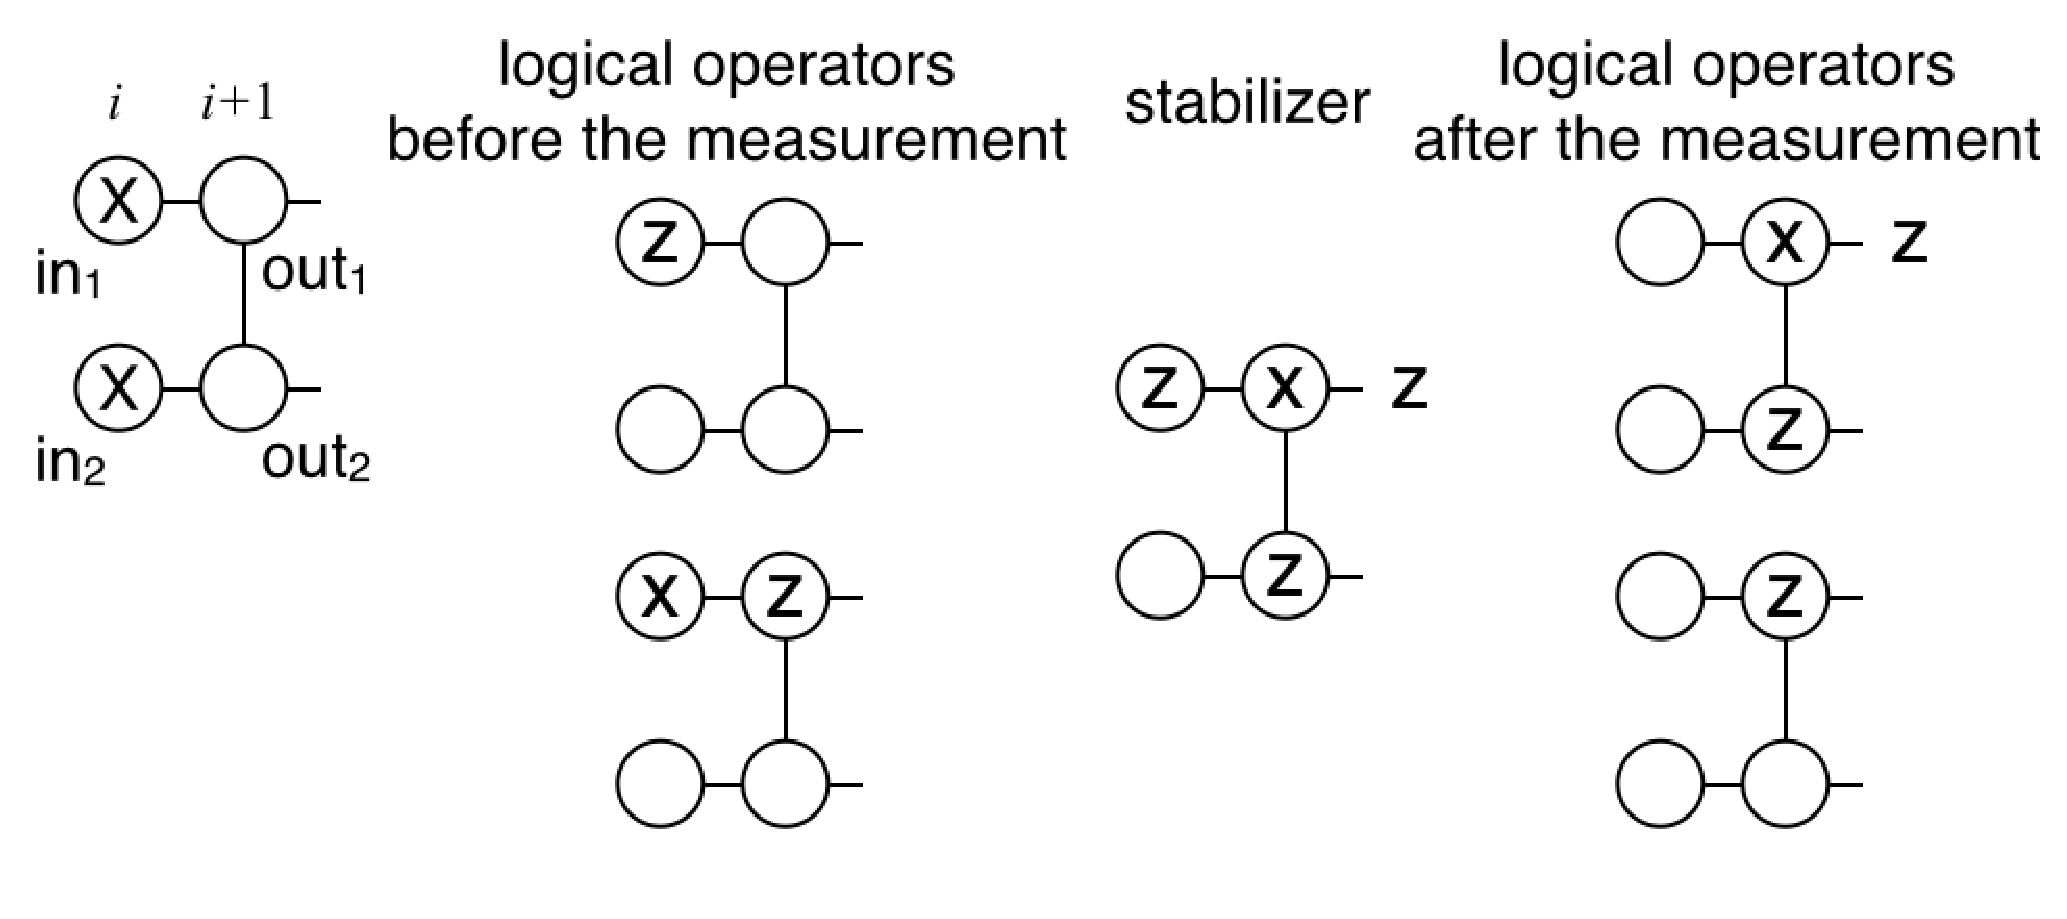
\includegraphics[width=110mm]{fig85.eps}
\end{center}
The logical operators for the $i$th step are given by $\{ L_{X1}^{(i)}, L_{Z1}^{(i)} \}$ and $\{ L_{X2}^{(i)}, L_{Z2}^{(i)} \}$.
By multiplying the stabilizer operator, we obtain
\begin{eqnarray}
L_{Z1}^{(i)} &\sim& X_{1,i+1} Z_{1,i+1} Z_{2,i+1} = L_{X1}^{(i+1)}L_{Z2}^{(i+1)}
,
\\
L_{Z2}^{(i)} &\sim& X_{2,i+1} Z_{2,i+1} Z_{1,i+1}= L_{X2}^{(i+1)}L_{Z1}^{(i+1)}
.
\end{eqnarray}
The logical operators for the $(i+1)$th step after the projections are calculated to be
\begin{eqnarray}
\{ L_{X1}^{(i)}, L_{Z1}^{(i)} \} \rightarrow \{ (-1)^{m_1} L_{Z1}^{(i+1)}, L_{X1}^{(i+1)}L_{Z2}^{(i+1)} \} = \{ VL_{X1}^{(i+1)}V^{\dag},VL_{Z1}^{(i+1)}V^{\dag} \},
\\
\{ L_{X2}^{(i)}, L_{Z2}^{(i)} \} \rightarrow \{ (-1)^{m_2} L_{Z2}^{(i+1)}, L_{X2}^{(i+1)}L_{Z1}^{(i+1)} \} = \{ VL_{X2}^{(i+1)}V^{\dag},VL_{Z2}^{(i+1)}V^{\dag} \}.
\end{eqnarray}
Again, we realize that the logical operators for the $i$th step are transformed into those for the $(i+1)$th step with a two-qubit unitary operation
\begin{eqnarray} 
V\equiv (X_1 Z_2)^{m_1} (X_2 Z_1)^{m_2} \Lambda_{1,2} (Z)H_1 H_2.
\end{eqnarray}
By combining single-qubit rotations $X^{m}He^{i (\theta/2) Z}$ and the two-qubit operation $ (X_1 Z_2)^{m_1} (X_2 Z_1)^{m_2} \Lambda_{1,2} (Z)H_1 H_2$ as seen above, we can perform a universal quantum computation. 
In this way, MBQC can be understood in the Heisenberg picture.

\begin{figure}[b]
\centering
%\sidecaption
% Use the relevant command for your figure-insertion program
% to insert the figure file.
% For example, with the option graphics use
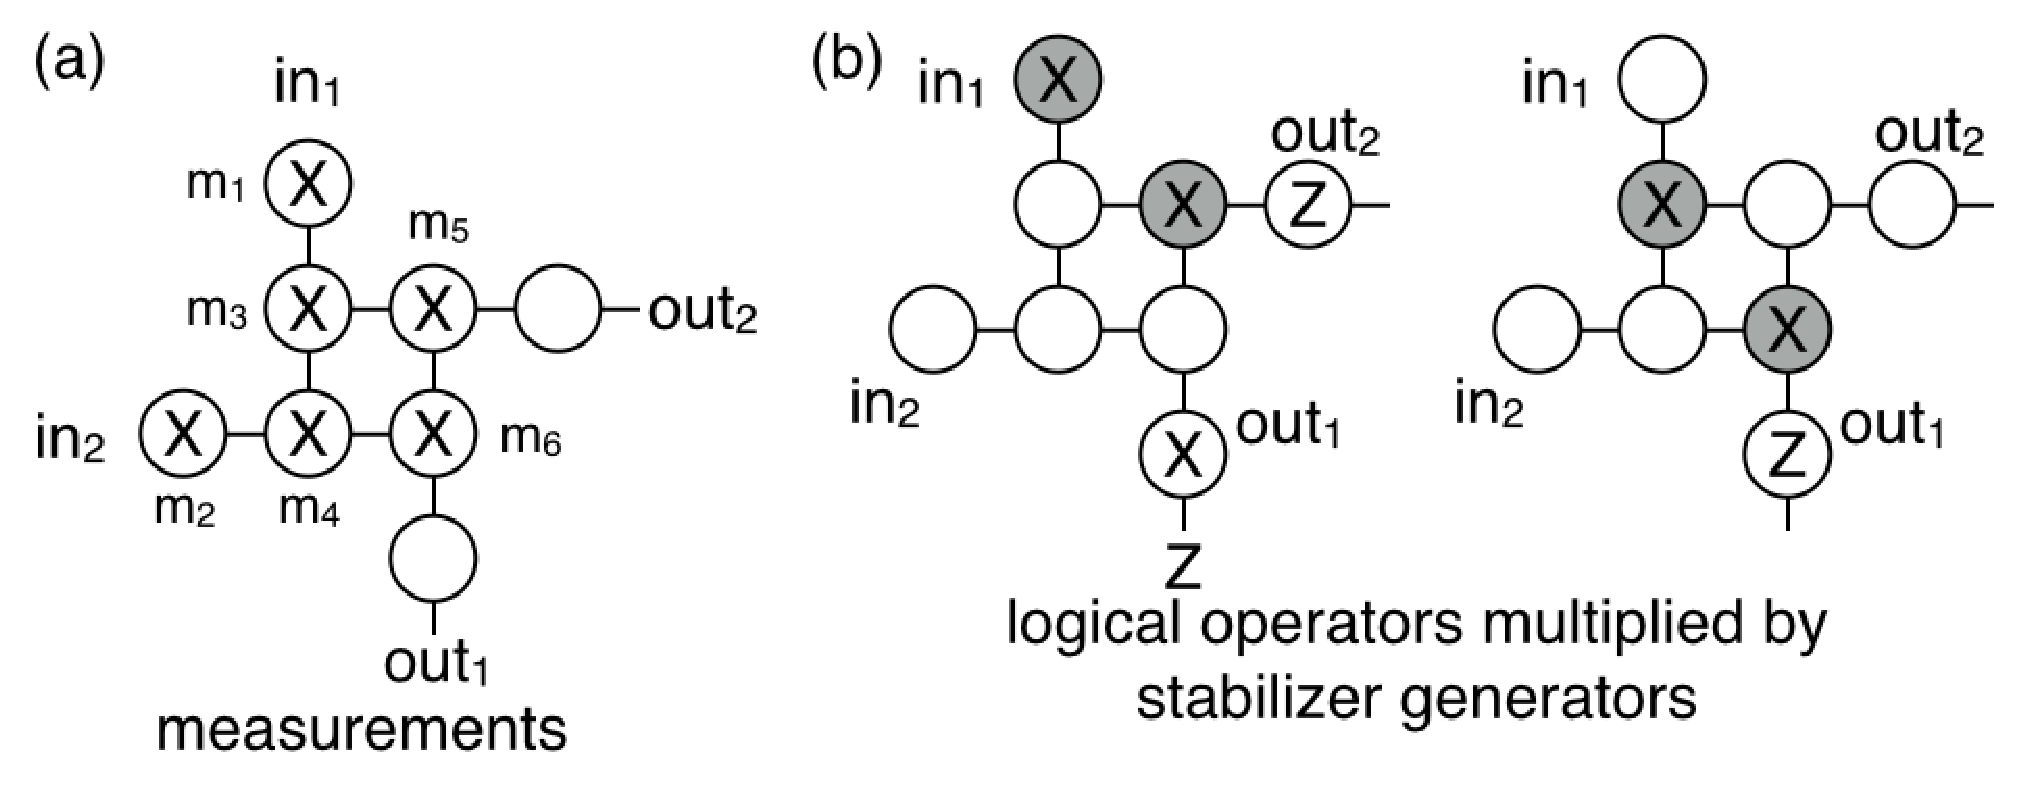
\includegraphics[width=120mm]{fig98.eps}
%
% If not, use
%\picplace{5cm}{2cm} % Give the correct figure height and width in cm
%
\caption{(a) A graph state and a measurement pattern.
(b) The logical $X$ operator of input 1 is multiplied by the stabilizer generators and we obtain a correlated operator on outputs 1 and 2 (left). 
The logical $Z$ operator of input 1 is multiplied by the stabilizer generators and we obtain the logical $Z$ operator of output 1.
The gray colored $X$ operators are replaced by $\pm1$ depending on the measurement outcomes.}
\label{fig98}       % Give a unique label
\end{figure}


Suppose the logical Pauli operators of the $k$th input and output qubits are related by the measurements as follows:
\begin{eqnarray}
\{ L_{X,k}^{({\rm In})}, L_{Z,k}^{(\rm In)} \}
\rightarrow 
\{ U L_{X,k}^{({\rm Out})} U^{\dag}, UL_{Z,k}^{(\rm Out)}U^{\dag} \}.
\end{eqnarray}
The unitary operator $U$ is performed on the input qubits.
Here a Pauli byproduct, depending on the measurement outcomes, is also included in $U$.
Moreover, if two graph states, which perform $U$ and $V$, are concatenated with the appropriate feedforwarding of the Pauli byproducts, then $VU$ is performed:
\begin{center}
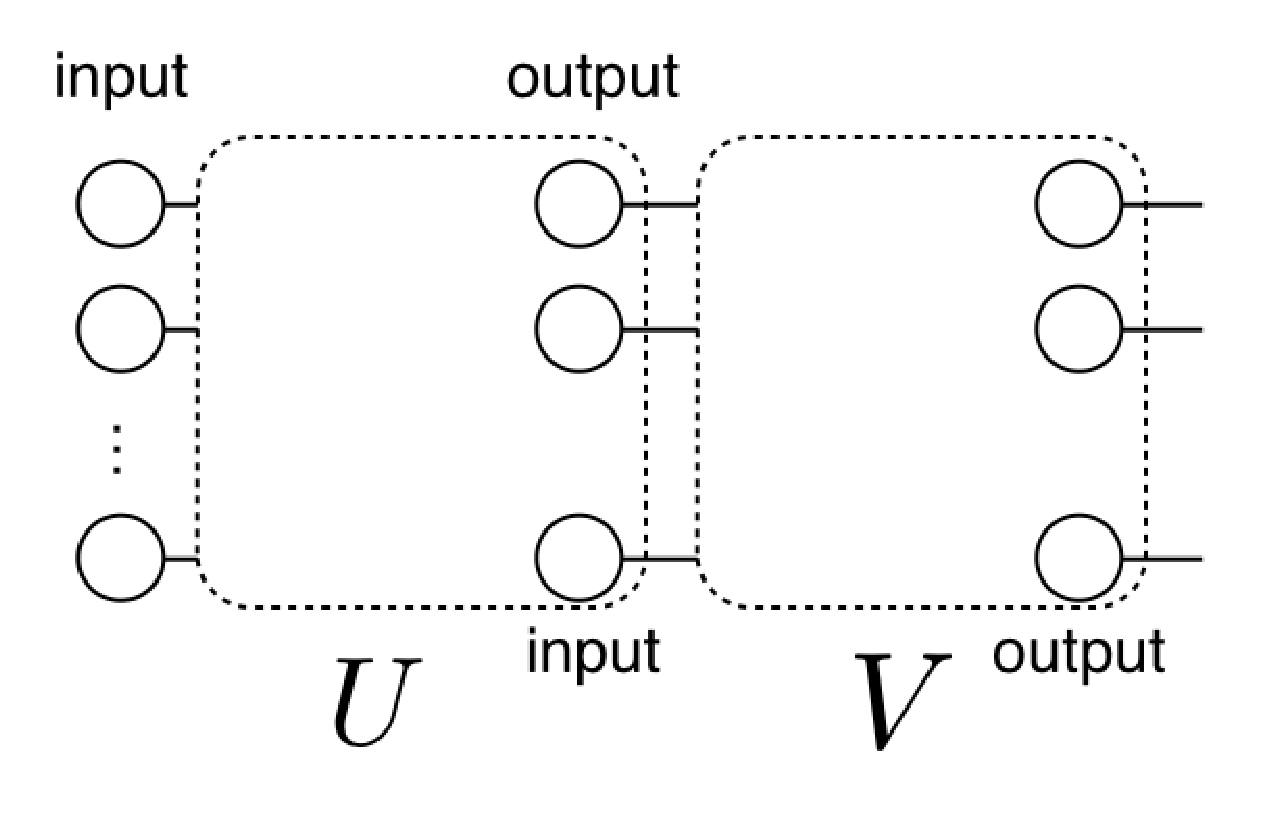
\includegraphics[width=70mm]{fig96.eps}
\end{center}

Let us consider the example shown in Fig.~\ref{fig98} (a).
The logical operators on the inputs are replaced by multiplying stabilizer generators so that they commute with the $X$-basis measurements.
Then the $X$ operators on the measured qubits are replaced by $\pm1$.
The measurements transform the input logical operators as follows:
\begin{eqnarray}
&&\{ L_{X,1}^{({\rm In})}, L_{Z,1}^{(\rm In)}, 
L_{X,2}^{({\rm In})}, L_{Z,2}^{(\rm In)} \}
\rightarrow 
\nonumber \\
&&\{ (-1)^{m_1 \oplus m_5} L_{X,1}^{({\rm Out})}L_{Z,2}^{({\rm Out})}, (-1)^{m_3 \oplus m_6}L_{Z,1}^{(\rm Out)}, 
(-1)^{m_2 \oplus m_6}L_{X,2}^{({\rm Out})} L_{Z,1}^{({\rm Out})} ,(-1) ^{m_4 \oplus m_5}L_{Z,2}^{(\rm Out)} \}.
\nonumber \\
\end{eqnarray}
Thus, the $\Lambda_{1,2}(Z)$ gate is implemented up to a Pauli byproduct.

Using this fact and concatenation of the input-output relations, we can construct a measurement-based CNOT gate between the separated two-qubit as follows~\cite{MBQC_PRA}:
\begin{center}
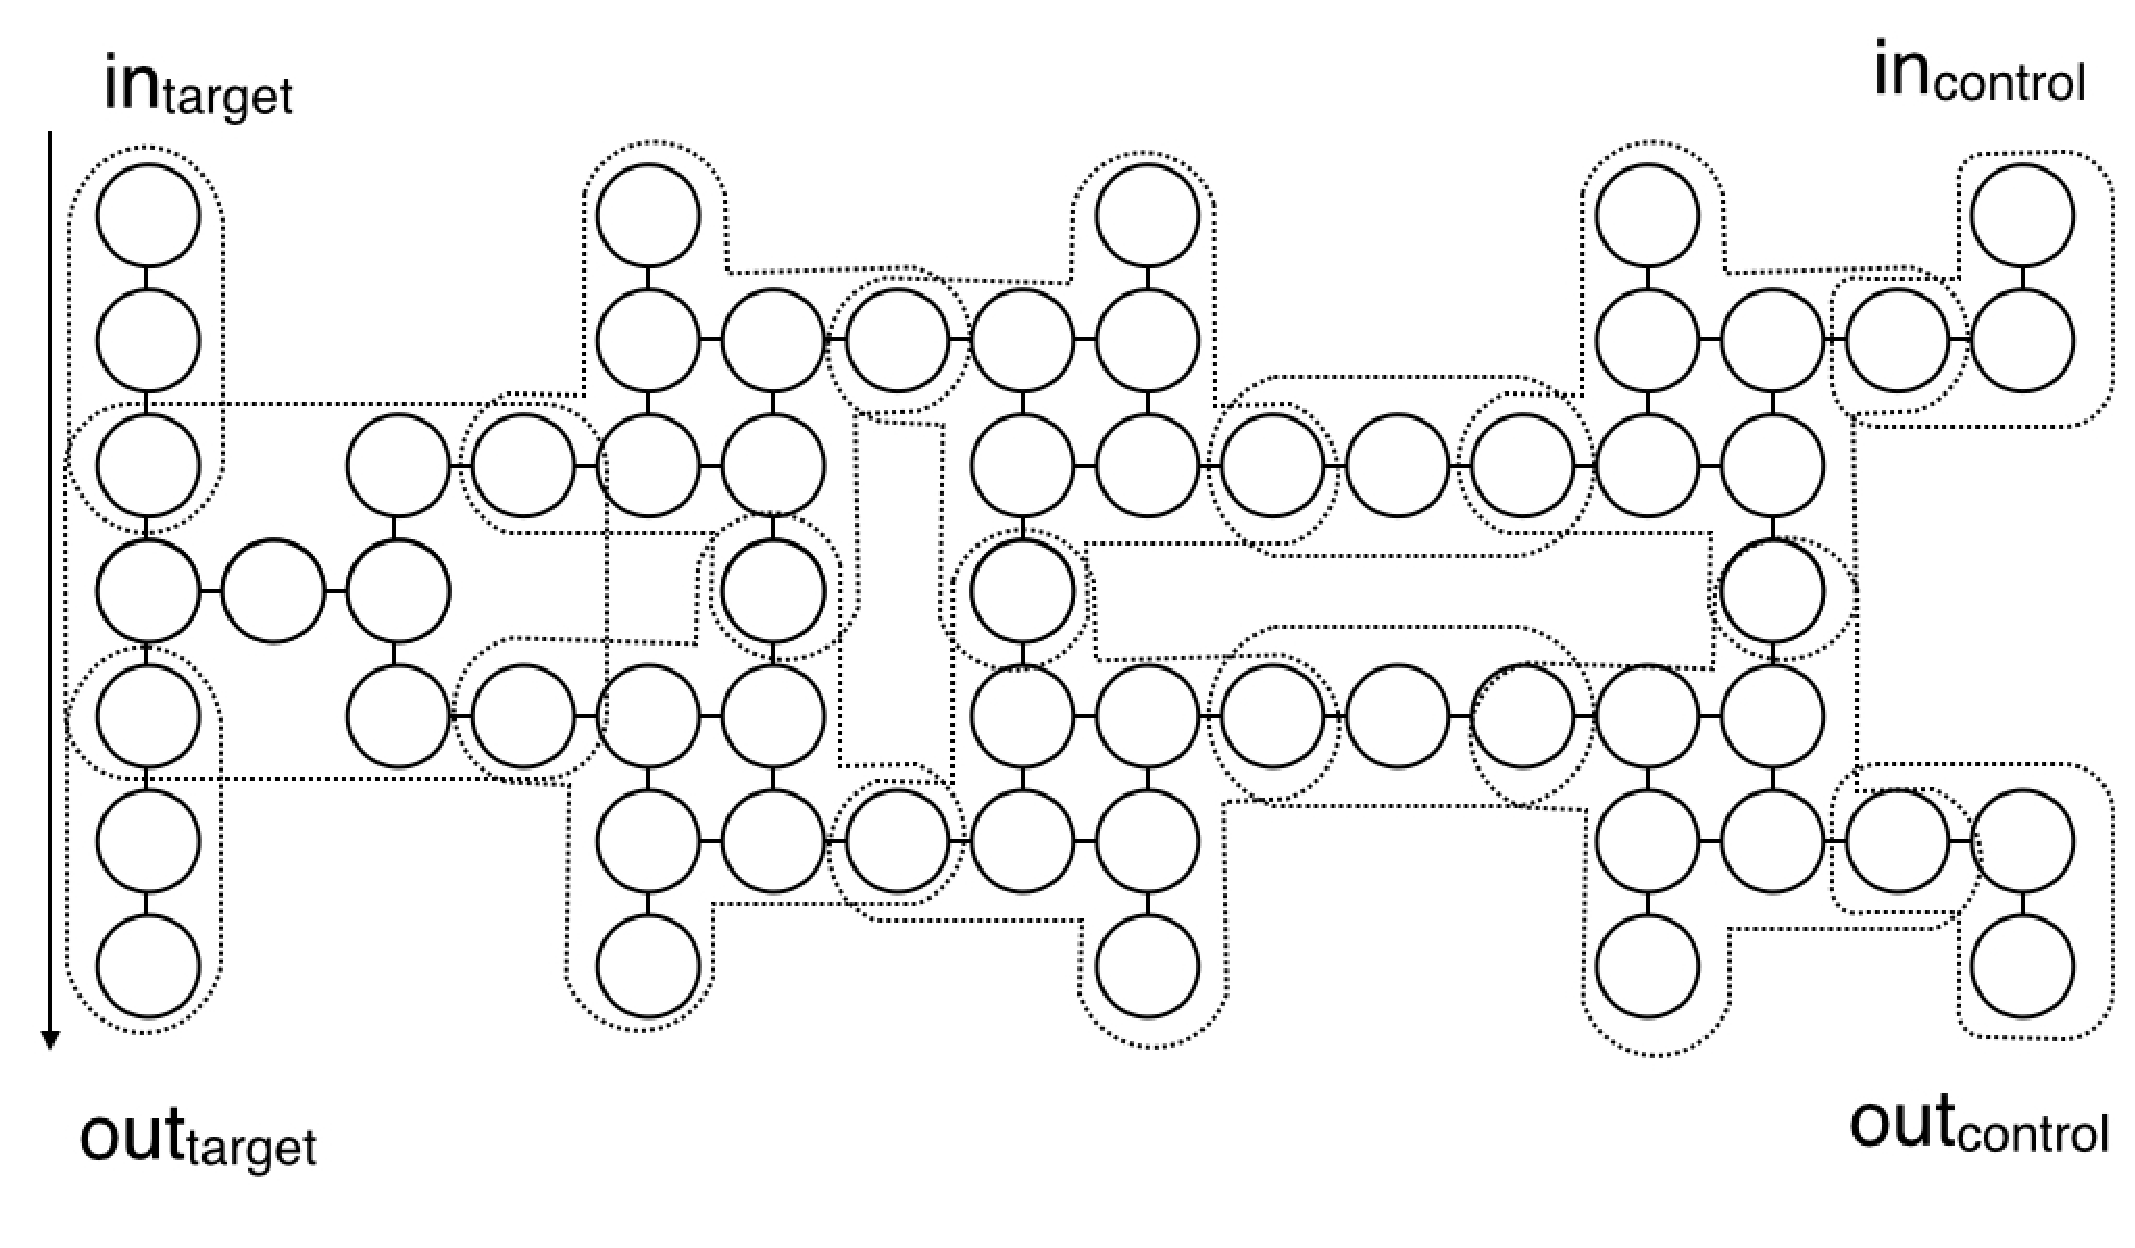
\includegraphics[width=90mm]{fig86.eps}
\end{center}
The input-output relation of the above graph state is equivalent to that for the following circuit:
\begin{center}
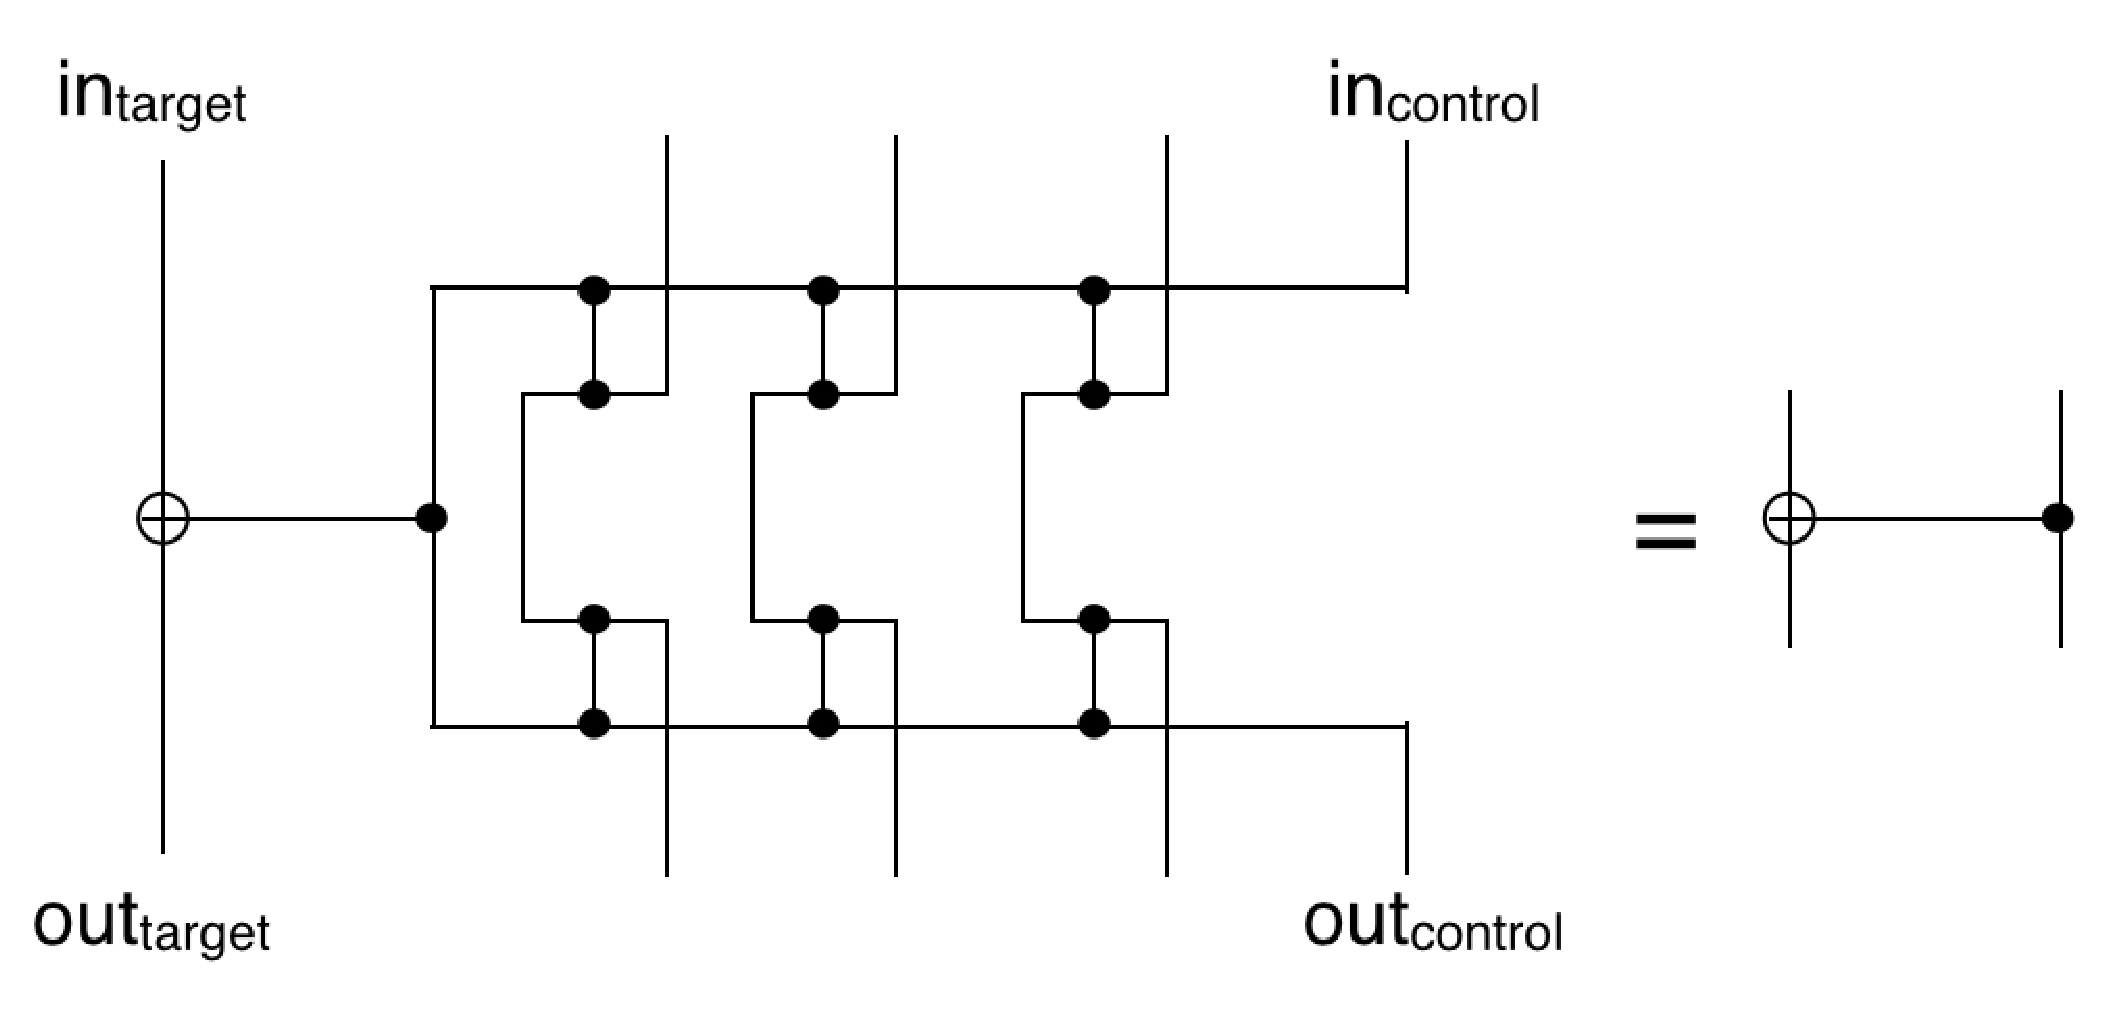
\includegraphics[width=90mm]{fig87.eps}
\end{center}
In this way, a CNOT gate between two arbitrary separated qubits can be implemented using a constant depth (constant width) resource state.

Topologically protected quantum computation was first proposed as a MBQC on a 3D cluster state~\cite{RaussendorfAnn,RaussendorfNJP}
as we will see in Chapter~\ref{Chap:TMBQC}.
It was further applied to the circuit-based model in two dimensions (2D)~\cite{RaussendorfPRL,FowlerHigh},
which will be explained in detail in Chapter~\ref{Chap:TQC}.
Specifically, in the formulations, the operator-based understanding is quite useful for tracking how correlation is propagated in a topologically protected way.
In Chapter~\ref{Chap:TMBQC}, we will formulate a topologically protected MBQC from the operator viewpoint and see how it is related to the circuit-based understanding explained in Chapter~\ref{Chap:TQC}.

To conclude, we summarize the properties of MBQC and recent progress in this area.
A unique feature of MBQC is that the resource state for universal quantum computation is prepared offline. 
Entangling operations, which would be one of the most difficult tasks in experiments, are employed only in this stage. 
Quantum computation is executed solely by adaptive measurements.
This property is useful for experimental realization in certain physical systems.
For example, a deterministic entangling operation is difficult to achieve in an optical quantum computation.
In such a case, we can utilize linear optics and measurement-induced nonlinearity to generate a cluster state~\cite{Yoran03,NielsenOpt,Browne05}.
Importantly, the entangling operation can be nondeterministic, as long as the successful or non-successful outcome is heralded.
By using such a probabilistic entangling operation, we can gradually expand the cluster state.
After successful cluster state generation, we can start the measurements for quantum computation.
Note that the probability of successful cluster state generation is not exponentially small by using a divide and conquer approach~\cite{NielsenOpt,Browne05,DuanRaussendorf,Matsuzaki10,LiBenjamin,FTProb}.

The clear separation between the quantum stage requiring entangling operations and the measurement stage is useful, not only for the physical implementation, but also in a quantum cryptographic scenario.
Suppose that Bob (server) possesses a fully fledged quantum computer and
that Alice (client), who has a less advanced quantum device, such as a single-qubit state generator, wants to delegate quantum computation to Bob.
By using the idea of MBQC, such a delegated quantum computation can be made unconditionally secure.
This is called a blind quantum computation and was proposed by Broadbent, Fitzsimons, and Kashefi (BFK)~\cite{Blind} (see also the related earlier works~\cite{ChildsBlind,ArrighiBlind}).
In the BFK protocol, Alice sends randomly rotated qubits $\{ e^{i \theta _j Z } |+\rangle\}$ to Bob, where the angle is chosen to be $\theta _j = k_j \pi /4$ ($k_j=0,1,...,7$).
Bob generates a cluster state by using the randomly rotated qubits.
In the computation phase, Alice sends a classical message $\delta _j = \phi _j + \theta _j + r_j \pi $.
Here, $\phi _j$ is the measurement angle with which Alice want to perform a measurement. The angle $\theta _j$ is for the randomly rotated state (which is secret to Bob). The random bit $r\in \{0,1\}$ makes the measurement angle completely random for Bob.
Then Bob performs the measurement in the $\{ e^{i\delta_j} |\pm \rangle\}$ basis.
Because the initial state is pre-rotated by $\theta_j$ (from Alice's viewpoint), Bob performs the measurement in the $\{ e^{i(\phi _j + r_j \pi) } |\pm \rangle\}$ basis, which is what Alice wants to do.
However, from Bob's viewpoint, the state is a completely mixed state with no information about $\{\phi _j\}$.
Thus, Bob is blind to any information about the input, the algorithm, and the output.
Instead of the state generation, Alice, who has a measurement device, can also perform a blind quantum computation, whose security is guaranteed by the no-signaling principle~\cite{MoriBlind}.
A fault-tolerant blind quantum computation has been proposed, based on topologically protected MBQC~\cite{BlindMoriFuji}.

\section{Quantum error correction codes}
In this section, we introduce stabilizer codes, which are a class of quantum error correction (QEC)\index{quantum error correction, QEC} codes.

\subsection*{Three-qubit bit-flip code}
The QEC codes can be  described elegantly in the stabilizer formalism.
Let us first consider the simplest one, the three-qubit bit flip code\index{three-qubit bit flip code}, whose stabilizer generators are given by
%
\begin{eqnarray}
S_{1} = Z_{1}Z_{2} , \;\;\; S_{2} = Z_{2}Z_{3}.
\end{eqnarray}
%
The stabilizer subspace is spanned by the following two logical states:
%
\begin{eqnarray}
|0_{L} \rangle = |000\rangle , \;\;\; |1_{L} \rangle=|111\rangle.
\end{eqnarray}
%
The logical Pauli-$X$ operator is given by $L_X \equiv X_{1}X_{2}X_{3}$.
The logical Pauli-$Z$ operator is defined as $L_Z\equiv Z_{1}$.
We may, equivalently, choose the logical Pauli $Z$ operator to be $Z_2$ or $Z_3$, because their actions on the code space are equivalent.
The present code is a quantum analogue of the classical three-bit repetition code.
Consider a bit flip error with an error probability $p$:
%
\begin{eqnarray}
\mathcal{E}_{i} \rho = (1-p) \rho + p X_{i} \rho X_{i}.
\end{eqnarray}
%
If the initial state $|\psi _{L} \rangle = \alpha|0_{L} \rangle +\beta |1_{L}\rangle $ undergoes the bit flip error independently, the output state is transformed in leading order as
%
\begin{eqnarray}
\mathcal{E} _{1} \circ \mathcal{E} _{2} \circ \mathcal{E} _{3}| \psi _{L} \rangle \langle \psi _{L} |
=  (1-p) ^3 | \psi _{L} \rangle \langle \psi _{L} |+p (1-p)^2 \sum_{i} X_{i} | \psi _{L}\rangle \langle \psi _{L} | X_{i} + O (p^2).
\nonumber \\
\label{eq:noise}
\end{eqnarray}
%
The error $X_i$ maps the code space to an orthogonal space.
We perform a projective measurement onto the orthogonal subspaces, $P_{k}^{\pm} = (I \pm S_{k})/2$, which we call a syndrome measurement, to know in which orthogonal space the state lies.
Note that the encoded quantum information is not destroyed by the syndrome measurement, because it commutes with the logical operators.
According to the measurement outcomes, the logical state can recover from the error as follows:
%
\begin{eqnarray}
\mathcal{R} \circ \mathcal{E} _{1} \circ \mathcal{E} _{2} \circ \mathcal{E} _{3}| \psi _{L} \rangle \langle \psi _{L} |
&=& [(1-p)^3 + 3p(1-p)^2 ] | \psi _{L} \rangle \langle \psi _{L} | + O(p^2),
\label{eq:recovery}
\end{eqnarray}
%
where the recovery operator is given by
%
\begin{eqnarray}
\mathcal{R} \rho &=& P_{1}^{+}P_{2}^{+} \rho P_{2}^{+}P_{1}^{+}+X_{1} P_{1}^{-}P_{2}^{+} \rho P_{2}^{+}P_{1}^{-} X_{1}+X_{2} P_{1}^{-}P_{2}^{-} \rho P_{2}^{-}P_{1}^{-} X_{2}
\nonumber \\
&&+X_{3} P_{1}^{+}P_{2}^{-} \rho P_{2}^{-}P_{1}^{+} X_{3}.
\end{eqnarray}
%
The four terms in $\mathcal{R}\rho$ correspond to the measurement outcomes (eigenvalues) $(+1,+1)$, $(-1,+1)$, $(-1,-1)$, and $(+1,-1)$
of the stabilizer generators, respectively.
By comparing Eqs.\ (\ref{eq:noise}) and (\ref{eq:recovery}), one can understand that if $p$ is sufficiently small, the fidelity of the logical state is improved.

Similarly, we can construct a three-qubit phase flip code\index{three-qubit phase flip code}, which can correct a phase flip error, by changing the basis with the Hadamard transformation:
\begin{eqnarray}
\langle Z_1 Z_2, Z_2 Z_3 \rangle \rightarrow \langle X_1 X_2 , X_2 X_3 \rangle.  
\end{eqnarray}

\subsection*{9-qubit Shor code}
The three-qubit bit-flip code cannot correct $Z$ errors, which commute with the stabilizer generators.
A QEC code that can correct all $X$, $Y$, and $Z$ errors was developed by Shor based on a concatenation of three-qubit bit-flip and phase-flip codes~\cite{Shor95}.
The stabilizer generators of the 9-qubit Shor code\index{9-qubit Shor code} are given as follows:
%
\begin{equation}
\begin{array}{ccccccccc}
\hline \hline
X & X & X& X& X& X & I & I & I
\\
I&I&I&X&X&X&X&X&X
\\
Z&Z&I&I&I&I&I&I&I
\\
I&Z&Z&I&I&I&I&I&I
\\
I & I & I & Z & Z & I & I & I & I
\\
I&I&I&I&Z&Z&I&I&I
\\
I&I&I&I&I&I&Z&Z&I
\\
I&I&I&I&I&I&I&Z&Z
\\
\hline \hline
\end{array}
\end{equation}
%
The code space is spanned by
%
\begin{eqnarray}
\frac{|0 _{L}\rangle + |1_{L} \rangle}{\sqrt{2}}
&=& 
\frac{\left(|000\rangle + |111 \rangle \right) \left(|000\rangle + |111 \rangle \right) \left(|000\rangle + |111 \rangle\right)}{2\sqrt{2}} ,  
\\
\frac{|0 _{L}\rangle - |1_{L} \rangle}{\sqrt{2}}
&=& 
\frac{\left(|000\rangle -|111 \rangle \right) \left(|000\rangle -|111 \rangle \right) \left(|000\rangle -|111 \rangle\right)}{2\sqrt{2}}.
\end{eqnarray}
%
The logical Pauli operators are given by $X_{L}=X^{\otimes 9}$ and $Z_{L}=Z^{\otimes 9}$, which are bitwise tensor products of physical Pauli operators.
If the logical $A$ operator is given by a bitwise tensor product of the physical $A$ operators on the QEC code, we say that the operation $A$ has {\it transversality}\index{transversality}.
The 9-qubit code is capable of correcting all $X$, $Y$, and $Z$ errors for each qubit, which can be understood because the three-qubit phase flip code 
$\{ |+++\rangle , |---\rangle \}$ is constructed by using the three logical qubits of the three-qubit bit flip codes $\{ |000\rangle, |111\rangle \}$.

Note that any single-qubit noise $\mathcal{E}$ can be described by using the Kraus operators $\{ K_j \}$:
\begin{eqnarray}
\mathcal{E} \rho = \sum _j K_j \rho K_j^{\dag}.
\end{eqnarray}
Any operator $K_j$ can be decomposed into the Pauli operators $\sigma _0 = I$, $\sigma _1=X$, $\sigma _2 = Y$, and $\sigma _3 =Z$:
\begin{eqnarray}
K_j = \sum _{l} c_{jl} \sigma _l.
\end{eqnarray}
Thus, if the $X$ and $Z$ errors on a single qubit are both corrected appropriately, we can correct any single-qubit noise automatically.
Specifically, because noise contains a superposition of the Pauli errors, it can be collapsed by the syndrome measurements.


\subsection*{Stabilizer codes}
To summarize the above examples, let us formalize the stabilizer quantum error correction codes and their properties. \index{stabilizer QEC code}
The code space of a stabilizer QEC code is defined by a stabilizer group $\langle \{ S_i \}\rangle$.
The encoded degree of freedom is specified by the mutually independent logical operators\index{logical operator} $\{L^{Z}_j\}$, which commute with all stabilizer generators and are independent of the stabilizer generators.
The computational basis state of the code state is completely determined by the stabilizer group $\langle \{ S_i\}, \{(-1)^{m_j} L^{Z}_j \} \rangle$.
We can always find another set of the logical operators $\{L^{X}_j\}$ being subject to
\begin{eqnarray}
L^X_j L^Z_i = (-1)^{\delta _{ij}} L^Z_i L^X_j ,
\end{eqnarray}
where $\delta _{ij}$ is the Kronecker delta.
Hence, the pair of logical operators $L_i^{Z}$ and $L_i^{X}$ represents the $i$th logical qubit\index{logical qubit}.
In terms of the numbers $n$ and $(n-k)$ of qubits and stabilizer generators, respectively, the number of pairs of logical operators is $k$. 

Let us define the {\it weight}\index{weight} ${\rm wt}(S_i)$ of a Pauli product $S_i$ as the number of qubits on which a Pauli operator (except for the identity $I$) is acting. 
The minimum weight of the logical operator over all possible logical operators is called the {\it code distance}\index{code distance} $d$. 
This implies that all Pauli products whose weights are smaller than $d$ are elements of the stabilizer group or anticommute with the stabilizer generators.
Thus, they act trivially on the code state	 or 
map the code state into an orthogonal subspace.
If the weight of a Pauli product as an error is less than $(d-1)/2$, we can find a unique recovery operator that returns the erroneous state into the code space.
Thus, we can correct weight-$\lfloor (d-1)/2 \rfloor$ errors.
Such a stabilizer QEC code is called a $[[n,k,d]]$ stabilizer code.
For example, the code distance of the 9-qubit code is a $[[9,1,3]]$ stabilizer code correcting weight-one errors.

The nine-qubit code is not the smallest QEC code that can correct all weight-one $X$, $Y$, and $Z$ errors.
The smallest code is the five-qubit code\index{five-qubit code}, found independently by Laflamme {\it et al.}~\cite{Laflamme96} and Bennett 
{\it et al.}~\cite{BCDSW96}.
The stabilizer generators and the logical Pauli operators are given as follows:
%
\begin{equation}
\begin{array}{cccccc}
\hline \hline
S_{1}=&X&Z&Z&X&I
\\
S_{2}=&I&X&Z&Z&X
\\
S_{3}=&X&I&X&Z&Z
\\
S_{4}=&Z&X&I&X&Z
\\
X_{L}=&X&X&X&X&X
\\
Z_{L}=&Z&Z&Z&Z&Z
\\
\hline \hline
\end{array}
\end{equation}
%
We see that the code distance is three, and hence an arbitrary single-qubit error can be corrected.


\subsection*{Calderbank-Shor-Steane codes}
The readers who are familiar with classical coding theory might already be aware of the correspondence between stabilizer codes and classical linear codes.
Let us recall the 9-qubit code.
The $X$ and $Z$ errors are detected independently through the $Z$-type and $X$-type stabilizer generators, respectively.
This implies that $X$ and $Z$ error corrections are described by classical coding theory, where two classical error corrections are subject to a certain constraint to appropriately form a stabilizer group.

To formulate this, we briefly review classical linear codes\index{classical linear code}.
A $[[n,k]]$ classical linear code $C$ is defined as a $k$-dimensional space $V_C$ over $GF(2^{n})$ by using an $n \times k$ generator matrix
\begin{eqnarray}
G=( \mathbf{b}_1 , ..., \mathbf{b}_k),
\end{eqnarray}
where the column vectors $\{ \mathbf{b}_i\}$ are the basis vectors of $V_C$. 
A $k$-bit classical information $\mathbf{y}$ is encoded into the code $\mathbf{c}$ as
\begin{eqnarray}
\mathbf{a}= G \mathbf{c}.
\end{eqnarray}
To detect and analyze the errors, we define an $(n-k)\times n$ parity check matrix\index{parity check matrix} $H$ such that $H \mathbf{b}_k=0$ for all basis vectors 
$\{ \mathbf{b}_k\}$.
Suppose an error $\mathbf{e}$ occurs on the code state, $\mathbf{a}' = \mathbf{a}\oplus \mathbf{e}$, where $\oplus$ indicates a bitwise addition modulo two.
By using the parity check matrix $H$, we can detect the error
\begin{eqnarray}
H \mathbf{a}'  = H(\mathbf{a} \oplus \mathbf{e})=H \mathbf{e}\equiv \mathbf{s},
\end{eqnarray}
where $\mathbf{s}$ is called an error syndrome.

For example, the three-bit repetition code is defined by the generator
\begin{eqnarray}
G = \left(\begin{array}{c}1 \\ 1 \\ 1 \end{array} \right).
\end{eqnarray}
A classical bit $0$ and $1$ is encoded into $(0,0,0)^{\rm T}$ and $(1,1,1)^{\rm T}$, respectively.
The parity check matrix is defined to be
\begin{eqnarray}
H= \left(
\begin{array}{ccc}
1 & 1 & 0
\\
0 & 1 & 1
\end{array}
\right).
\end{eqnarray}

Now, we realize that the positions of the 1s of the parity check matrix are exactly the same as those of the $Z$s in the stabilizer generators of the three-qubit bit flip code.
This suggests to use the parity check matrices $H_x$ and $H_z$ of the two classical linear codes $C_x$ and $C_z$, respectively, 
in the definition of the $X$-type and $Z$-type stabilizer generators:
\begin{eqnarray}
S_{X}^{(i)} = \prod _{j} X_j^{(H_x)_{ij}},
\;\;\;\;
S_{Z}^{(i)} = \prod _{j} Z_j^{(H_z)_{ij}}.
\end{eqnarray}
For these operators to commute with each other, the two parity check matrices have to satisfy
\begin{eqnarray}
H_x H_z^{\rm T} = \mathbf{0},
\end{eqnarray}
where $\mathbf{0}$ indicates a matrix with all elements $=0$.
To define the logical $Z$ operators, we define a quotient space ${\rm Ker}(H_x)/V_{H_z}:=\{ \mathbf{c}| H_x \mathbf{c} =0, \mathbf{c} \in V_{C_z} \}/V_{H_z}$, where $V_{H_z}$ is the space spanned by the column vectors of $H_{z}^{\rm T}$.
Denoting the basis vectors of the quotient space ${\rm Ker}(H_x)/V_{H_z}$ by $\{ [ \mathbf{b}_k^{z} ]\}$, we define the logical $Z$ operators
\begin{eqnarray}
L_Z^{(k)}=  \prod _{i} Z_i^{(\mathbf{b}^{z}_k)_i}.
\end{eqnarray}
Similarly, we can define the logical $X$ operators
\begin{eqnarray}
L_X^{(k)}=  \prod _{i} X_i^{(\mathbf{b}^{x}_k)_i},
\end{eqnarray}
using the basis vectors $\{ [\mathbf{b}_k^{x}] \}$ of a quotient space ${\rm Ker}(H_z)/V_{H_x}$, where $\mathbf{b}_k^{x}$ is chosen such that 
$L_Z^{(i)} L_X^{(j)} = (-1)^{\delta _{ij}}L_X^{(j)} L_Z^{(i)}$.
Note that dimensions of these kernel subspaces are the same, and we can easily find such pairs of anticommuting logical operators.
The above stabilizer code constructed from two classical linear codes is called a Calderbank-Shor-Steane (CSS) code\index{Calderbank-Shor-Steane code, CSS code}.

Let us see an important example of CSS codes, the 7-qubit code\index{7-qubit Steane code} introduced by Steane~\cite{Steane96}.
Specifically, we utilize a classical linear code, the $[[7,4,3]]$ Hamming code, whose generator and parity check matrices are given by
\begin{eqnarray}
G= \left( 
\begin{array}{cccc}
1 & 0 & 0& 0
\\
0 & 1 & 0 & 0
\\
0 & 0& 1 & 0
\\
0 & 0& 0& 1
\\
0 & 1 & 1 & 1 
\\
1 & 0 & 1 & 1 
\\
1 & 1 & 0 & 1
\end{array}
\right),
\;\;\;
H= \left( 
\begin{array}{ccccccc}
1 & 0 & 1 & 0 & 1 & 0 & 1
\\
0 & 1 & 1 & 0 & 0 & 1 & 1
\\
0 & 0 & 0 & 1 & 1 & 1 & 1
\end{array}
\right).
\end{eqnarray}
Because $H H^{\rm T}=\mathbf{0}$, we can employ the Hamming code to define both $X$- and $Z$-type stabilizer generators:
%
\begin{equation}
\begin{array}{cccccccccc}
\hline \hline
S_{1}&=& I&I&I&X&X&X&X
\\
S_{2}&=& I&X&X&I&I&X&X
\\
S_{3}&=& X&I&X&I&X&I&X
\\
S_{4}&=& I&I&I&Z&Z&Z&Z
\\
S_{5}&=& I&Z&Z&I&I&Z&Z
\\
S_{6}&=& Z&I&Z&I&Z&I&Z
\\
\hline
\hline
\end{array}
\end{equation}
There is an element $(1,1,1,1,1,1,1)^{\rm T}$ in the quotient space ${\rm Ker}(H)/V_H$.
The logical operators are given by
\begin{eqnarray}
\begin{array}{cccccccccc}
L_X&=& X&X&X&X&X&X&X,
\\
L_Z&=& Z&Z&Z&Z&Z&Z&Z.
\end{array}
\end{eqnarray}

The 7-qubit code is quite useful for fault-tolerant quantum computation.
Both the $X$- and $Z$-type stabilizer generators are defined from the Hamming code, and the stabilizer group is invariant under the transversal Hadamard operation 
$\bar H \equiv H^{\otimes 7}$.
Moreover, the logical $X$ operator is mapped into the logical $Z$ operator, $\bar H L_X \bar H = L_Z$.
Thus, the transversal Hadamard operation acts as the logical Hadamard operation for the encoded degree of freedom.
Similarly, a transversal phase operation $\bar S \equiv (ZS)^{\otimes 7}$ acts as a logical phase operation, $\bar S L_X \bar S^{\dag} =  L_X L_Y$.
Furthermore, a transversal CNOT operation $\bar \Lambda (X) = \Lambda(X)^{\otimes 7}$ keeps the stabilizer group of two logical qubits invariant:
\begin{eqnarray}
&&\langle \{ S_X^{(i)} \otimes I^{\otimes 7} \},
\{ S_Z^{(i)} \otimes I^{\otimes 7} \} ,
\{  I^{\otimes 7} \otimes S_X^{(i)} \},
\{  I^{\otimes 7} \otimes S_Z^{(i)} \} \rangle
\\
&&=
\langle \{ S_X^{(i)} \otimes S_X^{(i)} \},
\{ S_Z^{(i)} \otimes I^{\otimes 7} \} ,
\{  I^{\otimes 7} \otimes S_X^{(i)} \},
\{  S_Z^{(i)} \otimes S_Z^{(i)} \} \rangle.
\end{eqnarray}
The logical Pauli operators are subject to the transformation rule of the CNOT gate.
Accordingly, the transversal CNOT operation $\bar \Lambda (X)$ acts as a logical CNOT operation for the encoded degree of freedom.
Because the Hadamard, phase, and CNOT operations are implemented transversally, whole Clifford group elements can be implemented by transversal operations.

The transversal implementation is fault-tolerant because the operations apparently do not increase the number of errors on a code block and there is no internal interaction between the qubits in the same code block.
Combined with a fault-tolerant gadget for measuring the error syndrome as explained in Appendix~\ref{Ap:FT_syndrome_meas}, we can implement Clifford operations fault-tolerantly.

Unfortunately, the non-Clifford operation does not transform a Pauli operator into another Pauli operator.
For example, the $\pi/8$ operation $e^{ -i (\pi /8) Z}$ transforms the Pauli $X$ operator into a Clifford operator:
\begin{eqnarray}
e^{-i (\pi/8) Z} X e^{i (\pi/8) Z} = (X+Y)/\sqrt{2}.
\end{eqnarray}
This implies that a transversal non-Clifford operation hardly results in a logical non-Clifford operation.
Thus, a fault-tolerant non-Clifford gate operation is not so straightforward.
To settle this, we can utilize magic state distillation, consisting of noisy non-Clifford resource states and ideal (fault-tolerant) Clifford operations, as explained in the next section.


\section{Magic state distillation}
\label{sec:magic}
\subsection{Knill-Laflamme-Zurek protocol}
A fault-tolerant implementation of a non-Clifford gate was first proposed in an earlier paper by Knill, Laflamme, and Zurek~\cite{Knill98a,Knill98b}.
Instead of implementing the non-Clifford gate directly, we consider a fault-tolerant preparation of the non-stabilizer state, the so-called magic state\index{magic state},
\begin{eqnarray}
|A \rangle \equiv e^{ - i (\pi /8 ) Y }| +\rangle.
\end{eqnarray}
The magic state can be utilized to implement a non-Clifford gate $A \equiv e^{- i (\pi /8) Y}$ by using one-bit teleportation consisting of Clifford gates and the Pauli basis state preparations and measurements.
Thus, if we can prepare a clean magic state, we can create a fault-tolerant non-Clifford gate by using fault-tolerant Clifford gates.

The Knill-Laflamme-Zurek construction of the fault-tolerant preparation of the magic state was based on the fact that $|A\rangle$ is an eigenstate of $H$.
The Hadamard operation has transversality, e.g., on the 7-qubit code.
Hence, if we perform a projective measurement of $H^{\otimes 7}$, we obtain a clean magic state.
The circuit is given as follow
\begin{equation}
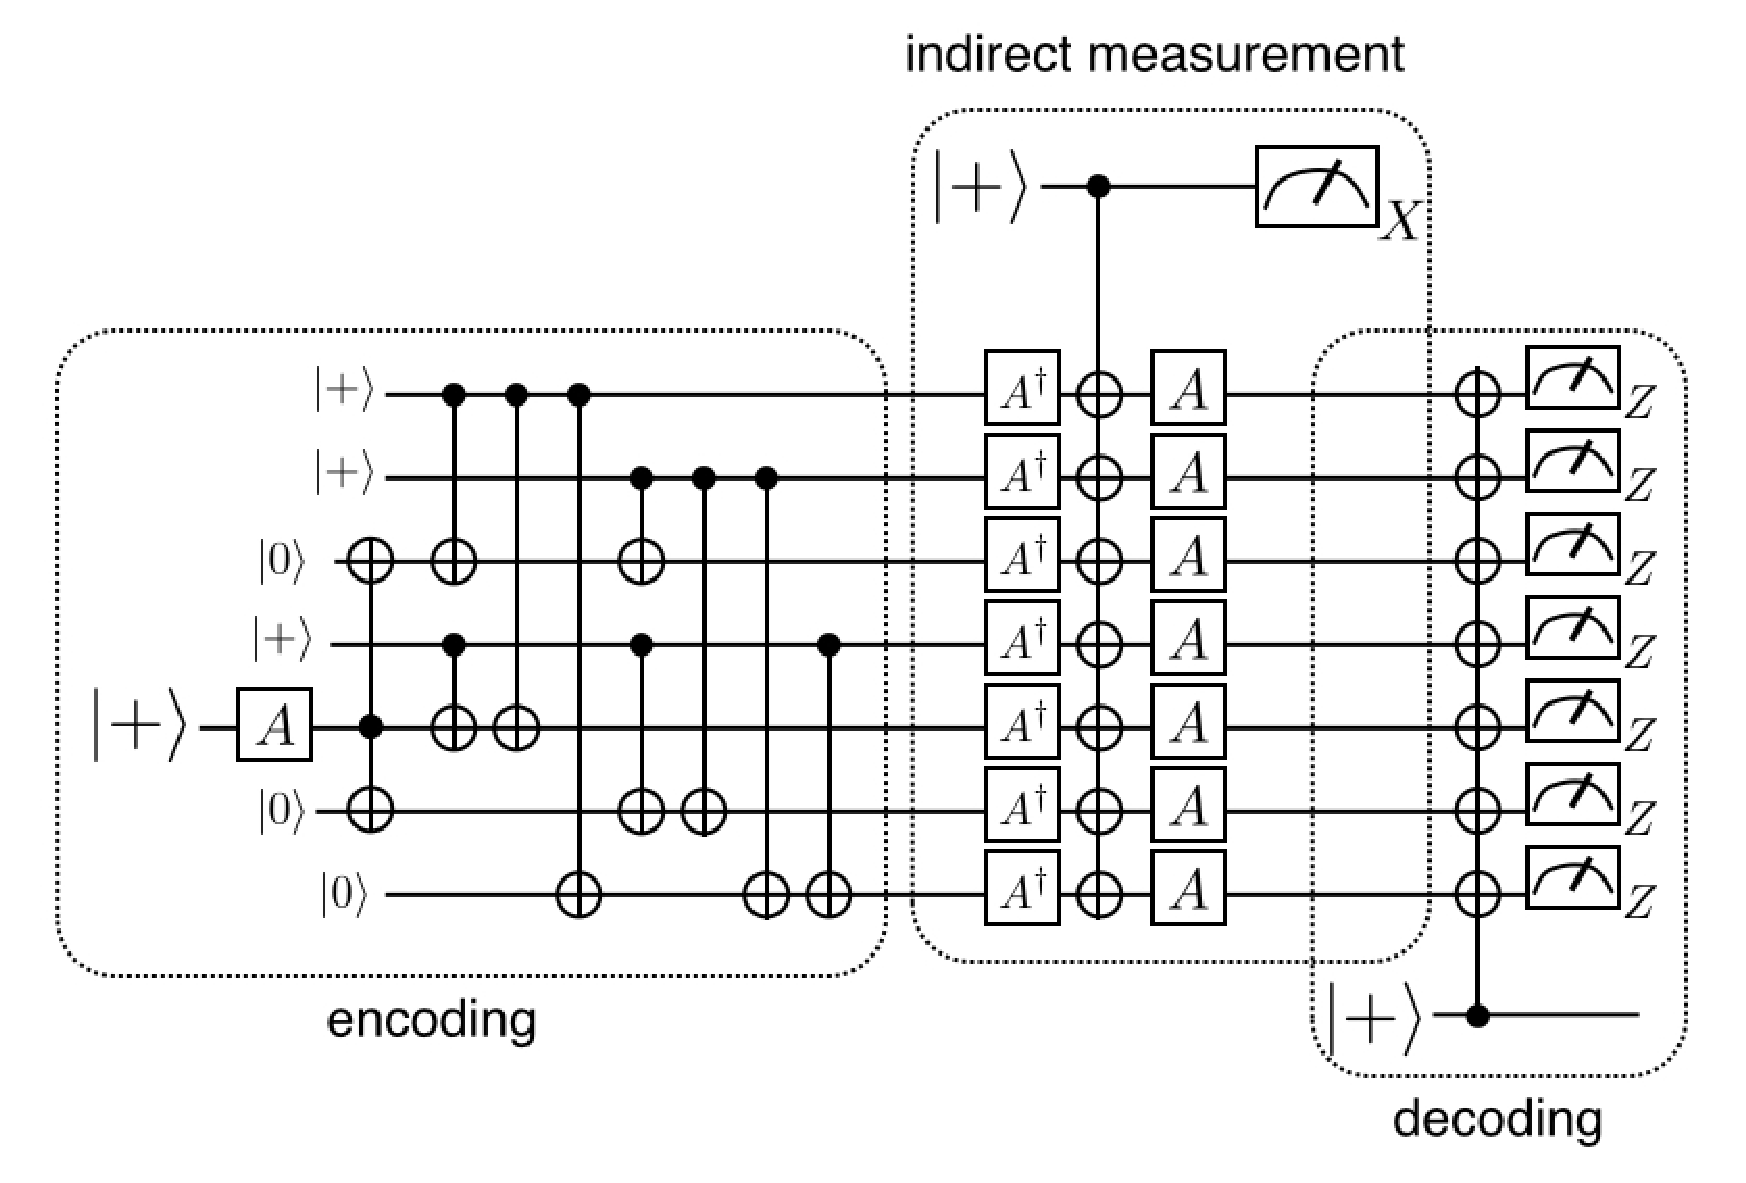
\includegraphics[width=120mm]{fig99.eps}
\end{equation}
where $A=e^{-i (\pi/8)Y}$ and we used the fact that $A_t \Lambda _{c,t}(X)A_t^{\dag}= \Lambda_{c,t}(H)$.
The above circuit consists of three parts, encoding of the logical magic state into the 7-qubit code, indirect measurement of $H^{\otimes 7}$, and decoding by one-bit teleportation.
Note that all Clifford operations are assumed to be ideal, because they are easily made fault-tolerant by using a stabilizer code.
With an appropriate randomization operation 
made up by Clifford operations, a noisy magic state can be transformed into a mixture of 
$|A\rangle$ and $|A^{\perp}\rangle = Y|A\rangle$:
\begin{eqnarray}
\rho _{A} = (1-p) |A\rangle \langle A| + p |A^{\perp}\rangle \langle A|
\end{eqnarray}
Hence, the noise on the magic state can be expressed as a $Y$ error.
The $Y$ error can be detected by transversal $Z$ measurements for the decoding (see also Knill's gadget for a fault-tolerant syndrome measurement in Appendix~\ref{Ap:FT_syndrome_meas}).
Assuming an ideal Clifford operation, the error probability $p$ decreases as $O(p^{3})$, when we employ the 7-qubit code with distance 3.
Including the $A$ gate for the initial encoding, we need 15 noisy magic states $|A\rangle$ to obtain a clean magic state.
This distillation protocol works for all self-dual CSS codes, which are symmetric between the $X$- and $Z$-type stabilizer generators and has transversality for the Hadamard gate.
Recently, improved protocols have been proposed based on this approach~\cite{Meier12,JonesMagic}.
 
 \subsection{Bravyi-Kitaev protocol}
Bravyi and Kitaev proposed another magic state distillation protocol based on a 15-qubit code~\cite{Magic}.
While their and the Knill-Laflamme-Zurek protocols seem quite different, they are, interestingly, known to be equivalent~\cite{Reichardt05}.
In the Bravyi-Kitaev protocol, a [[15,1,3]] quantum code is defined by the [[15,7,3]] classical Reed-Muller code\index{Reed-Muller code}, whose parity check matrix is given by
\begin{eqnarray}
H_x= \left( 
\begin{array}{ccccccccccccccc}
1 & 0 &0 &0 &0 &1 & 1& 0& 0& 1& 1 & 1& 1& 0 & 1
\\
0 & 1 & 0 & 0& 1 & 0 & 1 & 0 & 1 & 0 & 1 & 1 & 0 & 1 & 1 
\\
0 & 0 & 1 & 1 & 0 & 0 &1 & 0 & 1 & 1 & 0 & 0& 1 & 1 & 1 
\\
0 & 0& 1 & 0 & 1 & 1 & 0 & 1 & 0 & 0& 1 & 0& 1 & 1& 1
\end{array}
\right)
\end{eqnarray}
The $X$-type stabilizer generators are defined by $S_X^{(i)}= \prod _j X_j^{(H)_{ij}}$.
Then, we choose a parity check matrix of another classical code
\begin{eqnarray}
H_z= \left( 
\begin{array}{ccccccccccccccc}
0 & 0 &1 &1 &0 &0 & 0& 1& 0& 0& 0 & 0& 0& 0 & 1
\\
0 & 1 &0 &0 &1 &0 & 0& 1& 0& 0& 0 & 0& 0& 0 & 1
\\
1 & 0 &0 &0 &0 &1 & 0& 1& 0& 0& 0 & 0& 0& 0 & 1
\\
1 & 1 &0 &1 &0 &0 & 1& 0& 0& 0& 0 & 0& 0& 0 & 0
\\
0 & 1 &0 &1 &0 &0 & 0& 0& 1& 0& 0 & 0& 0& 0 & 1
\\
1 & 0 &0 &1 &0 &0 & 0& 0& 0& 1& 0 & 0& 0& 0 & 1
\\
1 & 1 &0 &0 &0 &0 & 0& 1& 0& 0& 1 & 0& 0& 0 & 0
\\
1 & 1 &0 &0 &0 &0 & 0& 0& 0& 0& 0 & 1& 0& 0 & 1
\\
1 & 0 &0 &1 &0 &0 & 0& 1& 0& 0& 0 & 0& 1& 0 & 0
\\
0 & 1 &0 &1 &0 &0 & 0& 1& 0& 0& 0 & 0& 0& 1 & 0
\end{array}
\right)
\end{eqnarray}
so that $H_x H_z^{\rm T}=\mathbf{0}$ and the $Z$-type stabilizer generators are defined similarly.
The logical operators are given by $L_X=X^{\otimes 15}$ and $L_Z=Z^{\otimes 15}$.
The logical states are written down explicitly as 
\begin{eqnarray}
|0_L\rangle 
&=& \prod _{i=1}^{4}(I+S_X^{(i)}) |00...0\rangle,
\\
|1_L\rangle 
&=& \prod _{i=1}^{4}(I+S_X^{(i)}) |11...1\rangle.
\end{eqnarray}
The number of 1s in each term of $|0_L\rangle$ and $|1_L\rangle$ is 8 and 7, respectively.
By applying the $T=e^{-i (\pi /8 )Z}$ gate transversally, we obtain
\begin{eqnarray}
T^{\otimes 15} |0 _{L}\rangle &=& e^{i \pi /8} |0 _{L}\rangle,
\\
T^{\otimes 15} |1 _{L}\rangle &=& e^{-i\pi/8} |0 _{L}\rangle.
\end{eqnarray}
Thus, the transversal $T$ gate acts as a logical $T^{\dag}$ gate.
Note that this transversality does not hold in the orthogonal (erroneous) subspace, e.g., spanned by $\{ X_k|0_L\rangle, X_k|1_L\rangle \}$.
However, we can show that this is enough to perform a fault-tolerant logical $T$ gate.

Instead of applying the $T$ gate directly, we implement it using a one-bit teleportation:
%
\begin{equation}
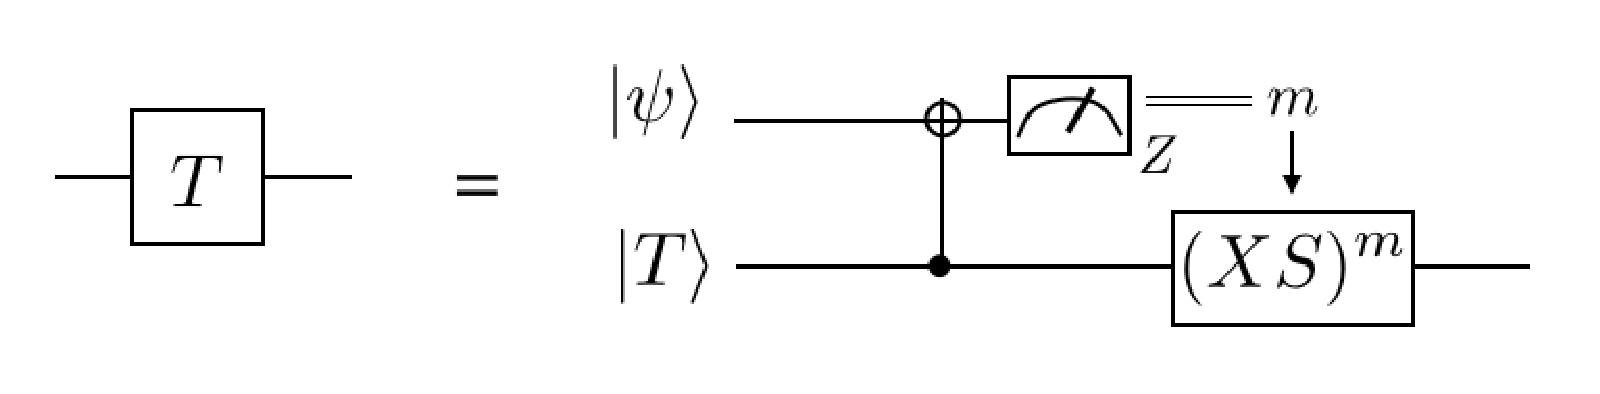
\includegraphics[width=110mm]{fig51.eps}
\end{equation}
%
The $Z$-basis measurement and CNOT operation are both implemented transversally on a CSS code.
Thus, if the preparation of the non-Clifford ancilla state $|T\rangle = (|0 _{L} \rangle + e^{-i \pi /4} |1_{L}\rangle)/\sqrt{2}$, called a magic state, is done fault-tolerantly, one can ensure fault-tolerance of the logical $T$ gate.

By using an appropriate randomization process, we can prepare a noisy magic state as follows:
\begin{eqnarray}
\rho _{T} = (1-p) |T\rangle \langle T| + p Z|T\rangle \langle T|Z.
\end{eqnarray}
Thus, a phase error $Z$ is located on the ideal magic state with probability $p$.
This phase error causes a $Z$ error after the $T$ gate by one-bit teleportation.
Because the code space is invariant under the transversal $T$ gate, we can detect such a $Z$ error by the following circuit.
\begin{center}
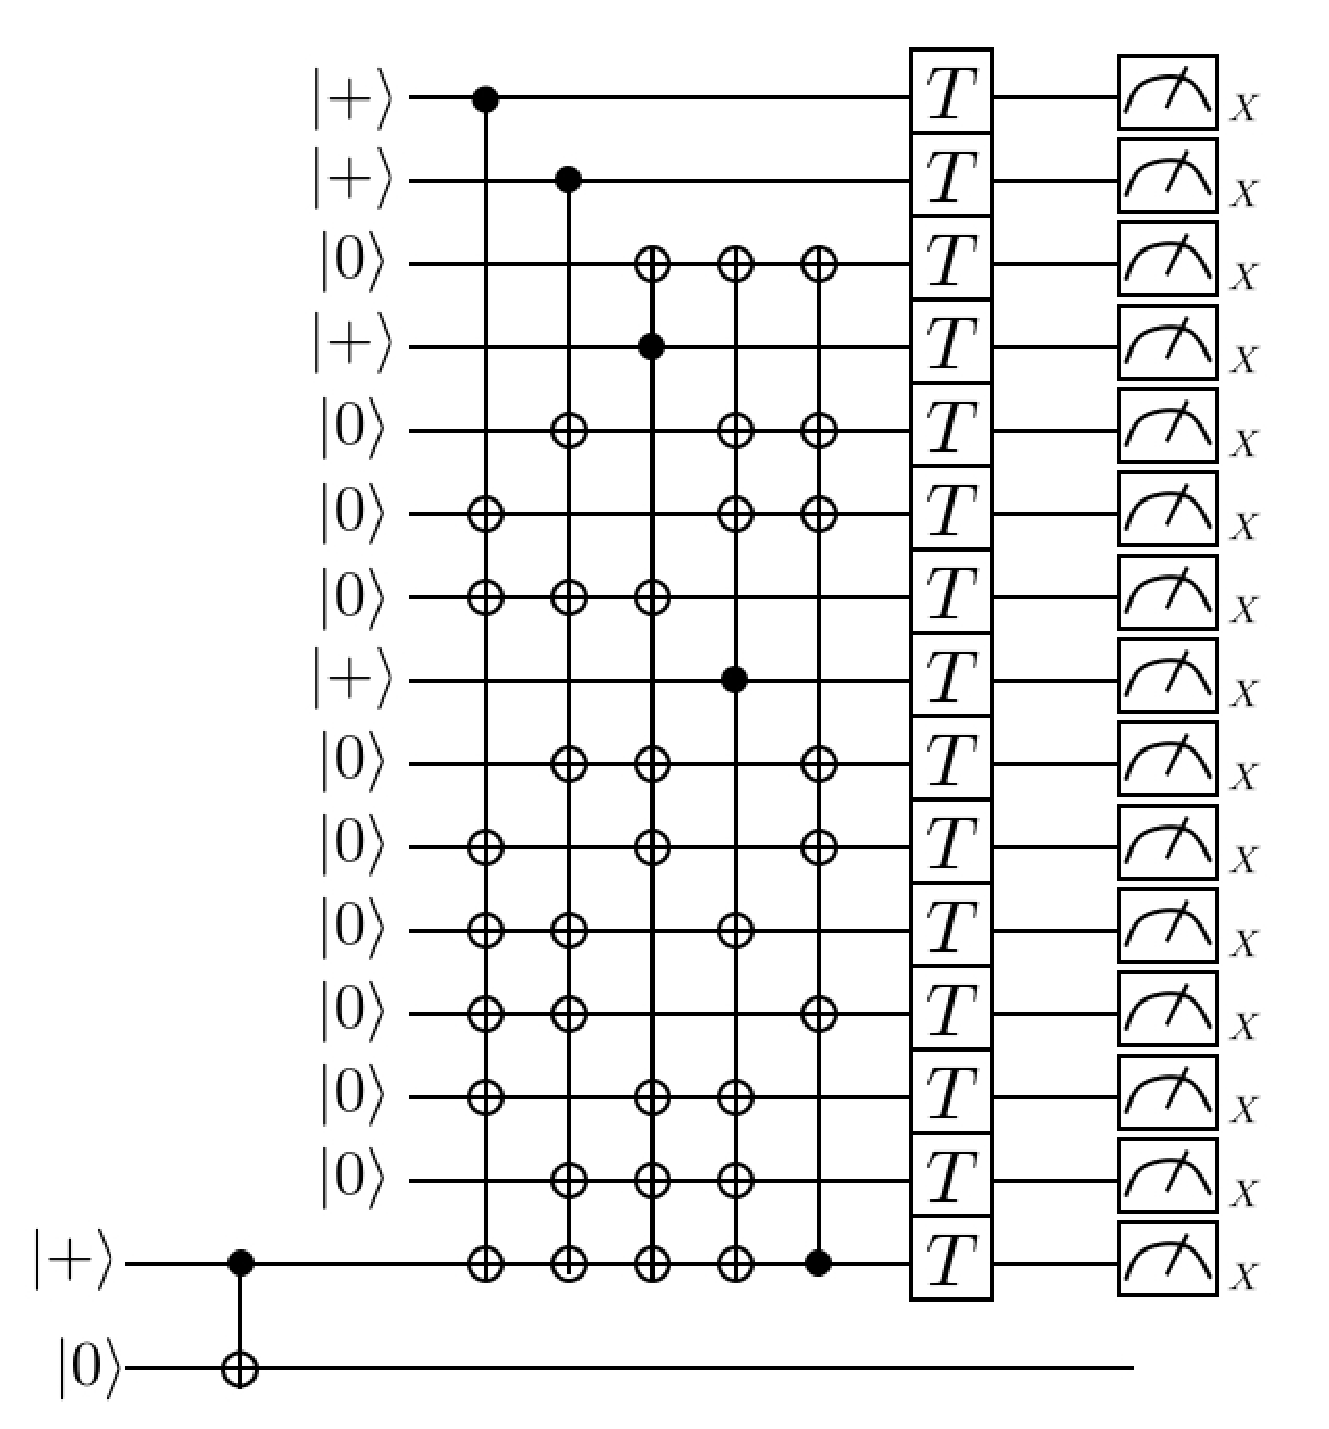
\includegraphics[width=90mm]{fig52.eps}
\end{center}
The first part of the above circuit consisting of CNOT operations is an encoding circuit for the quantum Reed-Muller code.
The transversal $T$ gate is applied by using one-bit teleportation.
The logical $|T\rangle$ state is measured in the $X$-basis transversally, which detects $Z$ errors on the code state, projecting the code state on the local $X$-basis.
The input state in the second lowest wire is entangled with the ancilla qubit in the lowest wire, where the distilled magic state is teleported.

Let $\mathbf{c}$ be a 15-bit string specifying the location of the $Z$ errors, $ E(\mathbf{c})\equiv \prod_i Z_i^{(\mathbf{c})_i}$.
If $E(\mathbf{c})$ commutes with the $X$-type stabilizer generators, the state passes through the distillation circuit.
To calculate this probability, we define a weight enumerator of a subspace $V \in GF(2^n)$,
\begin{eqnarray}
W_V(x,y)= \sum _{\mathbf{c} \in V} x^{n-{\rm wt}(\mathbf{c})} y^{{\rm wt}(\mathbf{c})}.
\end{eqnarray}
The probability of passing the distillation circuit is calculated to be
\begin{eqnarray}
p_{\rm pass}=W_{V_{H_x}^{\perp}}(1-p,p) = \frac{1}{|V_{x}|} W_{V_{H_x}}(1,1-2p) = \frac{1+15(1-2p)^8}{16} ,
\end{eqnarray}
where the orthogonal subspace $V_{H_x}^{\perp}$ is equivalent to the kernel of $H_x$, ${\rm Ker}(H_x)$. 
We also used the MacWilliams identity~\cite{macwilliams}:
\begin{eqnarray}
W_{V}(x,y)= \frac{1}{|V|} W_{V^{\perp}}(x+y,x-y).
\end{eqnarray}
Similarly, the error probability of the output can be calculated to be 
\begin{eqnarray}
W_{V_{H_z}}(p,1-p)&=&\frac{1}{|V_{H_z}^{\perp}|}W_{V_{H_z}^{\perp}}(1,2p-1) 
\\
&=& \frac{1+15(2p-1)^8+15(2p-1)^{7}+(2p-1)^{15}}{32}.
\end{eqnarray}
Accordingly, the error probability, under the condition of passing the distillation circuit, is given by
\begin{eqnarray}
p' = \frac{1+15(2p-1)^8+15(2p-1)^{7}+(2p-1)^{15}}{2[1+15(1-2p)^8]} = 35p^3+O(p^4).
\end{eqnarray}
If $p'>0.141$, we can reduce the error probability on the magic state via the distillation circuit.
After $l$ rounds of distillation, the error probability decreases to $(\sqrt{35} p)^{3^l}/\sqrt{35}$.
At each round, we need 15 noisy magic states. 
Because the probability of successfully passing the distillation circuit converges rapidly to 1, the average number of noisy magic states consumed after $l$ rounds becomes $15^{l}$.
Accordingly, the average number of noisy magic states required to achieve an error probability $\epsilon$ of the magic state scales like
\begin{eqnarray}
[\log (\sqrt{35} \epsilon)/ \log (\sqrt{35} p)]^{\log(15)/\log(3)} =O(\log ^{2.5} \epsilon).
\end{eqnarray}

In Sec.~\ref{sec:GKtheorem}, we saw that if an input state is a convex mixture of the Pauli basis states followed by Clifford operations and Pauli basis measurements, the measurement outcomes can be simulated classically in the weak sense.
The noisy magic state $\rho _{T} = (1-p) |T\rangle \langle T| + p |T\rangle \langle T|$ lies on a line in the $x$--$y$ plane, as shown in Fig.~\ref{fig53}.
\begin{figure}[t]
%\sidecaption
% Use the relevant command for your figure-insertion program
% to insert the figure file.
% For example, with the option graphics use
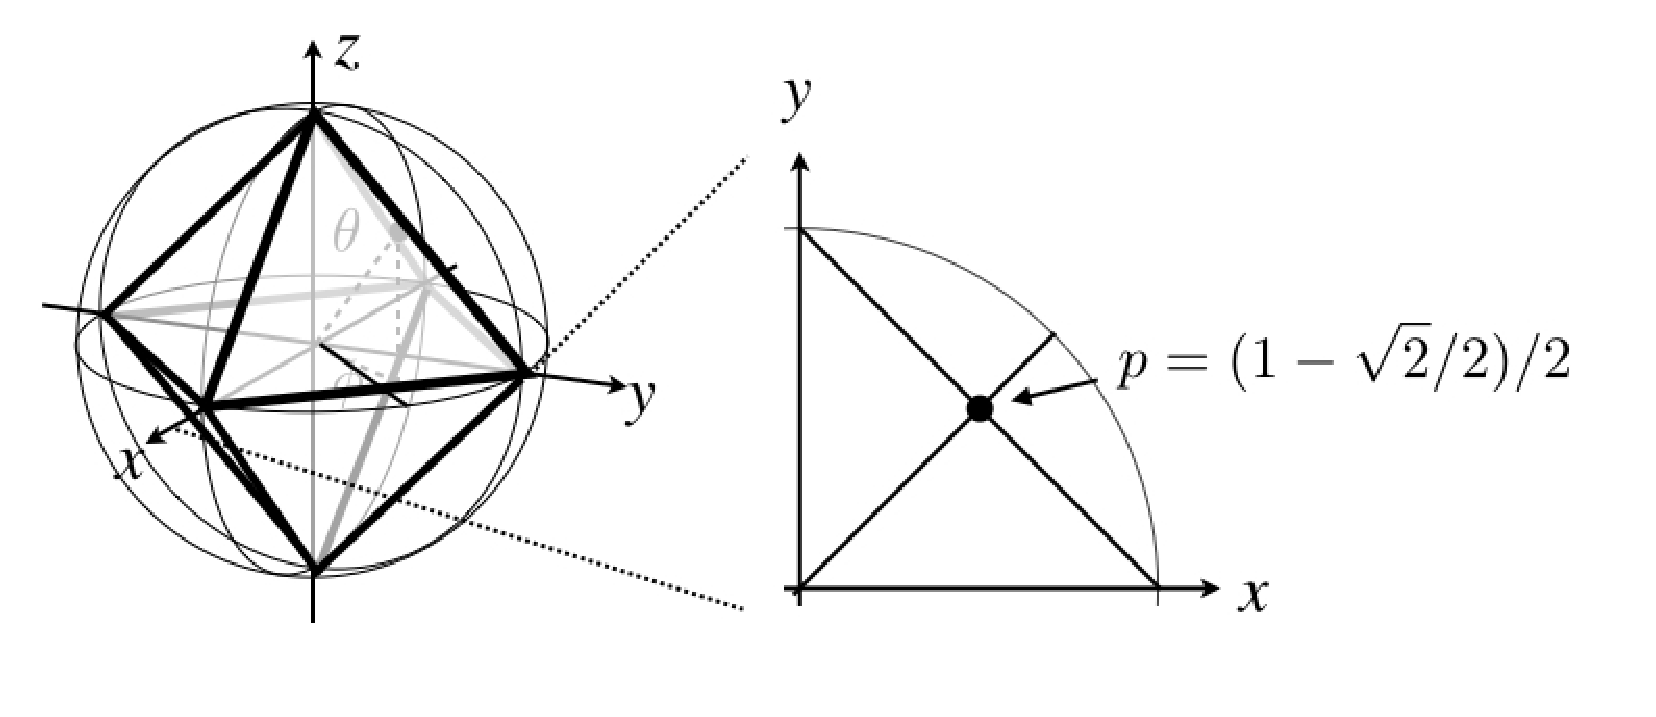
\includegraphics[width=120mm]{fig53.eps}
%
% If not, use
%\picplace{5cm}{2cm} % Give the correct figure height and width in cm
%
\caption{The noisy magic state in the Bloch sphere.}
\label{fig53}       % Give a unique label
\end{figure}
If $p > (1-\sqrt{2}/2)/2=0.146$, $\rho _{\pi/8}$ lies inside the octahedron, and the Gottesman-Knill theorem is applicable. 
On the other hand, if $p< 0.141$, magic state distillation allows us to implement universal quantum computation with an arbitrary accuracy as seen above.
Unfortunately, magic state distillation based on the Reed-Muller code does not provide a tight distillation threshold against the classically simulatable region.
In Ref.~\cite{Reichardt05}, a distillation protocol using the 7-qubit code was proposed and achieved a tight threshold $p=(1-\sqrt{2}/2)/2$.
In this sense, the classically simulatable and quantum universal regions 
are divided sharply on the $x$-$y$ plane.

By combining the magic state distillation and fault-tolerant Clifford operations on the CSS code, we can perform universal quantum computation fault-tolerantly.
In order to make the error probability arbitrarily small, we can employ concatenated quantum computation, in which logical qubits of a lower concatenation level are utilized as the physical qubits at a higher level.
At the higher level, all operations, including logical qubit preparations and syndrome measurements for QEC, have to be done fault-tolerantly.
If the error probability is smaller than a certain constant value, which we call the noise threshold, the logical error probability at the highest concatenation level decreases super-exponentially.
On the other hand, the overhead increases exponentially.
Thus, we can make the logical error probability small enough to maintain a quantum computation of size $N$ with a polylogarithmic overhead ${\rm polylog} (N)$.
This implies that we can obtain a quantum benefit even for a quantum algorithm with a quadratic speedup, such as the Grover algorithm~\cite{Grover}.
In Appendix~\ref{Ap:FT_syndrome_meas}, we briefly review fault-tolerant syndrome measurements, concatenated quantum computation, and the threshold theorem.

While the resource increment for protecting quantum computation scales polylogarithmically, its constant factor is quite huge.
Almost all overheads for the fault-tolerant quantum computation are employed for the magic state distillation~\cite{VanMeter,Jones12}. 
Thus, much effort has been spent recently on developing resource-efficient magic state distillation~\cite{Meier12,BravyiHaah,Eastin13,Jones13}. 